% !TeX spellcheck = en_US
\documentclass[preprint]{elsarticle}

\usepackage[left]{lineno}
\usepackage[latin1]{inputenc}
\usepackage[T1]{fontenc}
\usepackage{lmodern}
\usepackage{multirow}

\usepackage{lineno,hyperref}
\modulolinenumbers[5]

\usepackage[none]{hyphenat}

\usepackage{url}
\usepackage{booktabs}

\usepackage{tikz}
\usetikzlibrary{calc}
\usetikzlibrary{positioning}

\usepackage{mathtools}
\usepackage{amssymb}
\usepackage{amsthm}

\usepackage{caption}
\captionsetup{labelfont=bf}
\captionsetup{skip=0pt}

\usepackage{pgfplots}
\pgfplotsset{compat=newest}
\usepackage{algorithm}

\usepackage[noend]{algpseudocode}

\usepackage[margin=0.9in]{geometry}

\usepackage[normalem]{ulem}
%\usepackage{xcolor}

\newcommand{\Comentar}[1]{\State {\cmmt{#1}}}
\newcommand{\Break}{\State \textbf{break}}
\renewcommand{\Return}{\State \textbf{return}~}
\renewcommand{\algorithmicensure}{\textbf{Parameters:}}

\renewcommand\algorithmicthen{}
\renewcommand\algorithmicdo{}


\algblock{ForEach}{EndFor}
\algblock{ForDownTo}{EndFor}
\algblock{ForTo}{EndFor}

\newcommand{\Block}[1]{\State #1 \{}
\newcommand{\EndBlock}{\State \}}

\usepackage{scrextend}
\newcommand{\boldm}[1] {\mathversion{bold}#1\mathversion{normal}}
\newcommand{\round}[1]{\ensuremath{\lfloor#1\rceil}}
\usepackage{setspace}
\usepackage{array}
\usepackage{color, colortbl}
\usepackage{setspace} \doublespacing
\definecolor{Gray}{gray}{0.9}
\hyphenation{cost-ef-fec-tive-ness}

\newcommand{\specialcell}[2][c]{%
	\begin{tabular}[#1]{@{}c@{}}#2\end{tabular}}

\usepackage{textcomp}

\journal{Computers \& Industrial Engineering}


\begin{document}


\begin{frontmatter}

\title{Air cargo load and route planning in pickup and delivery operations}

%\author{A.C.P.~Mesquita}
%\ead{celio@ita.br}

%\author{C.A.A.~Sanches\corref{cor1}}
%\ead{alonso@ita.br}
%\cortext[cor1]{Corresponding author.}

%\address {Instituto Tecnol\'{o}gico de Aeron\'{a}utica - DCTA/ITA/IEC\\
%Pra\c{c}a Mal. Eduardo Gomes, 50\\
%S\~{a}o Jos\'{e} dos Campos - SP - 12.228-900 - Brazil}


\begin{abstract}

{\color{blue}In aerial pickup and delivery of goods in a distribution network, transport aviation faces risks of cargo unbalancing due to the urgency required for loading, immediate take-off, and mission accomplishment, especially in disaster relief, short deadlines, or any pressure for immediate take-off.}
In addition, there are no commercially available systems that can assist load and trip planners with pallet building and aircraft-balanced loading plans, with demands for transport at each hub. This enables other risks, such as improper delivery, excessive fuel burn, and longer than necessary turn-around time. We defined and solved the problem of planning the loading and routing of a single aircraft according to a utility score, weight and balance principles, and fuel consumption in a tour of simultaneous pickup and delivery at intermediate hubs. This {\it NP-hard}\/ problem, named {\it Air Cargo Load Planning with Routing, Pickup, and Delivery Problem (ACLP+RPDP)}, is mathematically modeled using standardized pallets in fixed positions, obeying center of gravity constraints, delivering each item to its destination, and minimizing fuel consumption costs. We performed multiple experiments with a commercial solver and four well-known meta-heuristics on data based on the transport history of the {\it Brazilian Air Force}. We also designed a new heuristic that quickly finds practical solutions to a wide range of problem sizes, a key contribution that resolved all real scenarios in much less time than is operationally acceptable.

\end{abstract}

\begin{keyword}
Load Planning \sep Air Palletization \sep Weight and Balance \sep Pickup and Delivery \sep Vehicle Routing
\end{keyword}

\end{frontmatter}

\label{sec1}
\section{Introduction}


Air cargo transport involves several sub-problems that are difficult to solve. Recently, Brandt and Nickel \cite[p. 401]{BrandtStefan2019} defined the {\it Air Cargo Load Planning Problem} (ACLPP) as four sub-problems: {\it Aircraft Configuration Problem} (ACP), {\it Build-up Scheduling Problem} (BSP), {\it Air Cargo Palletization Problem} (APP) and {\it Weight and Balance Problem} (WBP). Several aspects were considered in this modeling: characteristics of the items to be transported (dimensions, scores, dangerousness, etc.); types and quantities of {\it unit load devices} (ULDs), commonly called pallets; when these pallets are assembled; how items are allocated to pallets; in which positions these pallets are to be placed; how the total cargo weight is balanced; etc. They also presented a comprehensive bibliographic survey of solving methods that had been developed in different situations.

However, there are still other important challenges in air cargo transport that go beyond the definition of the ACLPP, especially with regard to the flight itinerary and the loading and unloading at each destination (or node) of this travel plan. In this context, at least two more important sub-problems can be considered: pickup and delivery operations at each node, called {\it Pickup and Delivery Problem} (PDP), and the search for the lowest cost route, which is the well-known {\it Traveling Salesman Problem} (TSP).

{\color{blue} Lurkin and Schyns \cite{LurkinSchyns2015} show that this problem is NP-hard and therefore compare their results to current manually generated solutions vice optimal (or even near optimal) solutions. They have shown that the WBP is also NP-hard.}

{\color{blue} Karp \cite{Karp1972} previously proved the 0-1 Knapsack problems to be NP-Hard, as the pallets may be seen as multiple knapsacks, the APP is also NP-hard. }

{\color{blue} Feng {\it et al.} (2015) \cite{Feng2015} presented a comprehensive literature assessment of commercial air cargo operations. They stated that the airplane loading problem is one of the fundamental issues in combinatorial optimization and described it as an NP-hard problem.}

There are real situations that are much more complex. In this work, we consider a practical case in Brazil, which is the largest economy in Latin America. Due to its dimensions, this country has the largest air market on the continent with $2,499$\/ registered airports, of which $1,911$\/ are private and $588$\/ are public. Although it is an immense distribution network, the {\it Brazilian Air Force}\/ missions have always considered 3 to 5 nodes per flight plan.

It is important to emphasize that this data is not an imposed limitation, but a historical fact that we will explore in our solution method. Throughout this work we approach routes with up to 7 nodes, as can be seen in Table \ref{tab:costs} and in Figure \ref{fig:nodes}. Although there are many other airports of interest to {\it Brazilian Air Force}, these 7 nodes were chosen due to their high demand and short transport times. The other Brazilian airports tend to have a lower demand, which is usually met, in a less expensive way, by cabotage, rail or road transport.


\begin{table}[H]
	
	\begin{minipage}{0.05\linewidth}
		
	\end{minipage}\hfill 
	\begin{minipage}{0.45\linewidth}
		
		\caption{Brazilian airports distances ($km$)}  \label{tab:costs}
		\centering
		\footnotesize
		\newcolumntype{Y}{>{\centering\arraybackslash}p{0.09\textwidth}}
		\newcolumntype{X}{>{\centering}p{0.09\textwidth}}
		
		\begin{tabular}{X X X X X X X Y}
			\toprule
			Node & $l_0$ & $l_1$ & $l_2$ & $l_3$ & $l_4$ & $l_5$ & $l_6$ \\
			IATA*   & GRU   & GIG   & SSA   & CNF   & CWB   & BSB   & REC \\	
			\midrule	
			GRU     & 0	    &343	&1,439   &504    &358    &866    &2,114\\
			GIG	    & 343	&0	    &1,218   &371    &677    &935    &1,876\\
			SSA	    & 1,439	&1,218	&0	    &938    &1,788   &1,062   &676\\
			CNF	    & 504	&371	&938	&0	    &851    &606    &1,613\\
			CWB	    & 358	&677	&1,788	&851	&0	    &1,084   &2,462\\
			BSB	    & 866	&935	&1,062	&606	&1,084	&0	    &1,658\\
			REC	    & 2,114	&1,876	&676	&1,613	&2,462	&1,658	&0\\
			\bottomrule
			\multicolumn{8}{c}{*International Air Transport Association}\\
			\multicolumn{8}{c}{\small\textsuperscript{Source: www.airportdistancecalculator.com}}\\
		\end{tabular}
		\normalsize
		
	\end{minipage}\hfill 
	\begin{minipage}{0.50\linewidth}
		\centering
		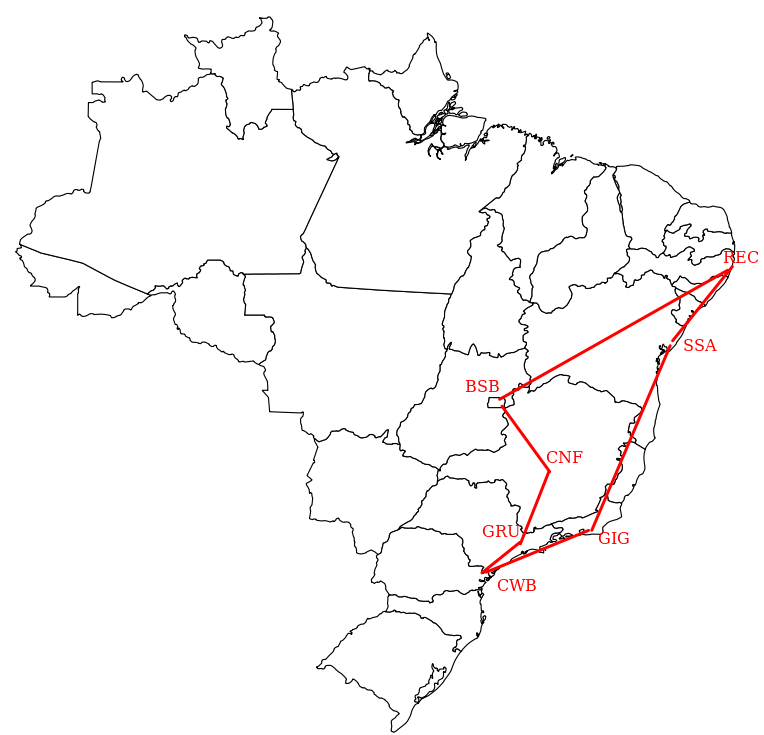
\includegraphics[scale=0.25]{Images/nodes.png}
		\captionof{figure}{A route with 7 Brazilian airports}
		\label{fig:nodes}
	\end{minipage}
\end{table}


Cargo handling at modern airports usually involves powerful equipment such as dollies, motorized conveyors, elevator transfer vehicles, caster decking, scissor lifts, electrical controls, hydraulically adjustable heights, forklift trucks, and plenty of room in the airport cargo terminal. These facilities, together with the use of standardized pallets with predefined positions on the aircraft, allow loading and unloading at each node to be carried out in about 30 minutes.

However, as reported by Fok and Chun, {\it load planning (...) is usually done in roughly 2 hours before departure, when all the details of the cargo are present.} \cite{fok2004optimizing}. We can infer that this is because adequate commercial software does not exist. In addition, there is still the necessary time to plan the route, in order to minimize fuel consumption and ensure the transport of priority items. In these circumstances, it is of great importance to find a method that speeds up the load planning and the definition of the flight itinerary.

Our work proposes a method that prioritizes the transport of the most relevant items at each node and the fuel economy along the tour. We developed a heuristic that can be run on a simple handheld computer (such as a laptop or a tablet) that previously defines a flight plan, and provides a quick solution for cargo handling. Consequently, this method reduces the stress that transport planners are subjected to, because they have to deal with a lot of information in planning the aircraft route, assembling the pallets (regarding their positions), and a pick up and delivery plan to each node.

To the best of our knowledge, this is the first time that an air cargo transport problem that simultaneously involves APP, WBP, PDP and TSP has been addressed. This new problem is named {\it Air Cargo Load Planning with Routing, Pickup and Delivery Problem} (ACLP+RPDP).

This article is organized into six more sections. In Section \ref{sec2}, we give a brief review of the literature. In Section \ref{sec3}, we present the problem context and assumptions, and in Section \ref{sec4}, we describe the mathematical model and how we dealt with its issues. In Section \ref{sec5}, we describe the elaborate algorithms, whose results are presented in Section \ref{sec6}. Finally, our conclusions are in Section \ref{sec7}.

\section{Related literature}
\label{sec2}

{\color{blue} In this section, we briefly describe the characteristics of the main works related to air cargo transport, following the chronological order of Table \ref{tab:sa}, that lists the main works in the literature and the corresponding sub-problems addressed. We also indicate whether the dimensions of the items were taken into account ({\bf 3D} or {\bf 2D}) and which solution method was used: heuristic search methods ({\bf Heu}), integer programming ({\bf Int}), or linear programming ({\bf Lin}). }

\begin{table}[H]
	\centering
	\caption{Air cargo transport: literature, problems and features}  \label{tab:sa}
	\scriptsize
	\renewcommand{\arraystretch}{1.1} 
	\begin{tabular}{r|cccc|ccccc}
		\toprule
		Work & {\bf APP}  & {\bf WBP}  &  {\bf PDP}   &{\bf TSP}   & {\bf 2D}  & {\bf 3D}  & {\bf Heu}  & {\bf Int}  & {\bf Lin} \\
		\midrule
		Larsen and Mikkelsen \cite{LarsenMikkelsen1979}  & $.$        & $\bigstar$ & $.$          & $.$        & $.$       & $.$       & $\bigstar$ & $.$        &  $.$ \\
		Brosh \cite{Brosh1981}  & $.$ & $\bigstar$  & $.$   & $.$ & $.$ & $.$   & $.$  & $.$  &  $\bigstar$ \\
		Ng \cite{Kevin1992}  & $.$ & $\bigstar$  & $.$ & $.$ & $.$ &$.$   & $.$  & $\bigstar$  &  $.$ \\
		Heidelberg {\it et al.} \cite{Heidelberg1998}  & $.$ & $\bigstar$  & $.$ & $.$ & $\bigstar$ &$.$   & $\bigstar$  & $.$  &  $.$ \\
		Mongeau and Bes \cite{MongeauBes2003}    & $\bigstar$ & $\bigstar$   & $.$ & $.$ & $.$ & $.$   & $.$  & $\bigstar$  &  $.$ \\
		Fok and Chun \cite{fok2004optimizing} & $.$ & $\bigstar$   & $.$ & $.$ & $.$ & $.$   & $.$  & $\bigstar$  &  $.$ \\	
		Chan {\it et al.} \cite{Chan2006}  & $\bigstar$ & $.$    & $.$ & $.$ & $.$ & $\bigstar$  & $\bigstar$  & $.$  &  $.$ \\
		Kaluzny and Shaw \cite{KaluznyBohdanL2009Oalb}  & $.$ & $\bigstar$  & $.$  & $.$ & $\bigstar$ &$.$  & $.$  & $\bigstar$  &  $.$ \\
		Verstichel {\it et al.} \cite{Verstichel2011}   & $.$ & $\bigstar$    & $.$ & $.$ & $.$ & $.$   & $.$  & $\bigstar$  &  $.$ \\
		Mesquita and Cunha \cite{MesquitaCunha2011}   & $.$ & $.$    & $\bigstar$ & $.$ & $.$ & $.$   & $\bigstar$  & $.$  &  $.$ \\		
		Limbourg {\it et al.} \cite{Limbourg2012} & $.$ & $\bigstar$  & $.$ & $.$ & $.$ & $.$   & $.$  & $\bigstar$  &  $.$ \\
		Roesener and Hall \cite{RoesenerHall2014}  & $\bigstar$ & $\bigstar$  & $.$  & $.$ & $.$ & $\bigstar$   & $.$  & $\bigstar$  &  $.$ \\
		Vancroonenburg {\it et al.} \cite{Vancroonenburg2014}  & $\bigstar$ & $\bigstar$   & $.$ & $.$ & $.$ & $.$   & $.$  & $\bigstar$  &  $.$ \\
		Lurkin and Schyns \cite{LurkinSchyns2015} & $.$ & $\bigstar$  & $\bigstar$ & $.$  & $.$ & $.$   & $.$  & $\bigstar$  &  $.$ \\
		Roesener and Barnes \cite{RoesenerBarnes2016}  & $.$ & $\bigstar$   & $.$ & $.$ & $.$ & $.$   & $\bigstar$  & $.$  &  $.$ \\
		Paquay {\it et al} \cite{PaquaySchynsLimbourg2016,PaquayLimbourgSchynsOliveira2018}  & $\bigstar$ & $\bigstar$ & $.$ & $.$ & $.$ & $\bigstar$ & $\bigstar$  & $\bigstar$ & $.$ \\
		Chenguang {\it el al.} \cite{YangLiuGao2018} & $.$ & $\bigstar$  & $.$  & $.$ & $\bigstar$  & $.$ & $\bigstar$ & $.$  & $.$ \\
		Wong and Ling \cite{wong2020} & $\bigstar$  & $\bigstar$  & $.$  & $.$   & $.$  & $.$ & $.$ & $\bigstar$  & $.$  \\
		Wong {\it et al.} \cite{eugene2021} & $\bigstar$ & $\bigstar$ & $.$  & $.$   & $.$ & $.$ & $.$ & $\bigstar$  & $.$  \\
		Zhao {\it et al.} \cite{zhao2021} & $.$ & $\bigstar$ & $.$  & $.$  & $.$ & $.$ & $.$  & $\bigstar$ &  $.$ \\
		
		{\color{blue}		Zhao {\it et al.} } \cite{zhao2023} & $\bigstar$ & $\bigstar$ & $.$  & $.$  & $.$ & $.$ & $.$  & $\bigstar$ &  $.$  \\
		
		{\bf This article}   & $\bigstar$ & $\bigstar$  & $\bigstar$& $\bigstar$ & $.$ & $.$ & $\bigstar$ & $\bigstar$   &  $.$  \\
		\bottomrule 
	\end{tabular}
	\normalsize 
\end{table}


As can be seen, so far Lurkin and Schyns \cite{LurkinSchyns2015} is the only work that simultaneously addresses an air cargo (WBP) and a flight itinerary (PDP) sub-problem. Although it is innovative, strong simplifications were imposed by these authors: in relation to loading, APP was ignored; with regard to routing, it is assumed a predefined tour plan restricted to only two legs. It is important to note that these authors consider an aircraft with two doors, and the minimization of loading and unloading costs at the intermediate node was modeled through a container sequencing problem. Referring directly to this work, Brandt and Nickel \cite[p. 409]{BrandtStefan2019} comment: {\it However, not even these sub-problems are acceptably solved for real-world problem sizes or the models omit some practically relevant constraints}. 



Larsen and Mikkelsen \cite{LarsenMikkelsen1979} developed an interactive procedure for loading 14 types of Boeing 747 into a two-leg transportation plan. Seven types of items were considered to be allocated in 17 to 42 positions. With non-linear programming and heuristics, they present a solution that minimizes positioning changes in the intermediate node, optimizing the load balancing in the aircraft.

Brosh \cite{Brosh1981} addressed the problem of planning the allocation of cargo on an aircraft. Considering volume, weight and structural constraints, the author finds the optimal load layout through a fractional programming problem.

Ng \cite{Kevin1992} developed a multi-criteria optimization approach to load the {\it C-130} aircraft of the {\it Canadian Air Force}. Based on integer programming, this model provides timely planning and improves airlift support for combat operations, solving WBP with pallets in fixed positions, and considering 20 different items.

Heidelberg {\it et al.} \cite{Heidelberg1998} developed a heuristic for 2D packing in air loading, comparing it with methods for solving the {\it Bin Packing Problem}. These authors conclude that the classical algorithms are inadequate in this context, because they ignore the aircraft balancing constraints.

Mongeau and Bes \cite{MongeauBes2003} presented a method based on linear integer programming to solve the problem of choosing and positioning containers in the {\it Airbus 340-300}. Safety and stability constraints were considered, with the objective of minimizing fuel consumption.

Fok and Chun \cite{fok2004optimizing} developed a web-based application to make efficient use of space and load balancing for an air cargo company. Based on an analysis of historical data, an operational load planning with mathematical optimization is obtained. This container load planning is usually done in roughly 2 hours before departure, when all cargo details are in place.

Chan {\it et al.} \cite{Chan2006} carried out a case study with heterogeneous pallets. To minimize the total cost of shipping, they developed a 3D packing heuristic, with a loading plan for each pallet. Although the authors do not consider load balancing or positioning of pallets in the cargo hold, this method is relevant in commercial and industrial applications, where cargo items tend to be less dense.

Kaluzny and Shaw \cite{KaluznyBohdanL2009Oalb} developed a mixed integer linear programming model to arrange a set of items in a military context that optimizes the load balance. The objective function can be chosen to minimize the deviation of the center of gravity (CG) from the target position or to maximize the function of the items loaded. This approach does not palletize items, which are arranged in the cargo bay by a 2D packing procedure.

Verstichel {\it et al.} \cite{Verstichel2011} solved WBP by selecting the most profitable subset of containers to be loaded into an aircraft by the use of mixed-integer programming. Experimental results on real-life data showed significant improvements compared to those obtained manually by an experienced planner.

Mesquita and Cunha \cite{MesquitaCunha2011} presented a heuristic for a real problem of the {\it Brazilian Air Force}, which consists of defining transport routes with simultaneous collection and delivery from a central distribution terminal.

Limbourg {\it et al.} \cite{Limbourg2012} developed a mixed-integer program for optimally rearranging a set of pallets into a compartmentalized cargo aircraft, specifically the {\it Boeing 747}.

Roesener and Hall \cite{RoesenerHall2014} solved APP and WBP as an integer programming problem, where the items are selected for shipment based on a utility score, then assigned to pallets, which will be loaded into an aircraft in a specific pallet position.
The pallets are then packed in a manner to optimize both the pallet and aircraft characteristics, such as item utility, pallet occupancy, and aircraft center of balance.
This method groups items by destinations to be served by multiple aircraft.

Vancroonenburg {\it et al} \cite{Vancroonenburg2014} presented a mixed integer linear programming model that selects the most profitable pallets, satisfying safety and load balancing constraints on the {\it Boeing 747-400}. Using a solver, these authors solved real problems in less than an hour.

As already mentioned, Lurkin and Schyns \cite{LurkinSchyns2015} was the first work that simultaneously modeled WBP and PDP in air cargo transport. The authors demonstrated that this problem is NP-hard and performed some experiments with real data, noting that their model offers better results than those obtained manually.


Roesener and Barnes \cite{RoesenerBarnes2016} proposed a heuristic to solve the {\it Dynamic Airlift Loading Problem} (DALP). Given a set of palletized cargo items that require transport between two nodes in a time frame, the objective of this problem is to select an efficient subset of aircraft, partition the pallets into aircraft loads and assign them to allowable positions in those aircraft.

Paquay {\it et al.} \cite{PaquaySchynsLimbourg2016} presented a mathematical modeling to optimize the loading of heterogeneous 3D boxes on pallets with a truncated parallelepipeds format. Its objective is to maximize the volume used in containers, considering load balancing constraints, the presence of fragile items and the possibility of rotating these boxes. Paquay {\it et al.} \cite{PaquayLimbourgSchynsOliveira2018} developed some heuristics to solve this problem.

Chenguang {\it et al.} \cite{YangLiuGao2018} modeled the air transport problem as a 2D packing problem, and presented a heuristic for its optimization in several aircraft, considering load balancing to minimize fuel consumption.

Wong and Ling \cite{wong2020}A�developed a mathematical model and a tool based on mixed integer programming for optimizing cargo in aircraft with different pallet configurations. Balance constraints and the presence of dangerous items were considered. Wong {\it et al.} \cite{eugene2021} integrated this tool to a digital simulation model, with a visualization and validation system, based on sensors that alert about load deviations.

Zhao {\it et al.} \cite{zhao2021} proposed a new modeling for WBP based on mixed integer programming. Instead of focusing on the CG deviation, the authors consider the original CG envelope of the aircraft, with a linearization method for its non-linear constraints.

{\color{blue} Zhao {\it et al.} \cite{zhao2023}  proposed three integer linear programming models: a Bi-objective Optimization Model (BOM), a Combinatorial Optimization Model (COM), and an Improved Combinatorial Optimization Model (IOM). The objectives of their solutions were the maximum loading capacity and the lowest CG deviation from a specified target CG. Four scenarios with various conditional metrics for three models are solved for the B777F aircraft using Gurobi. The results of the computations demonstrated that the BOM has the fastest solution speed, but the CG deviation is the largest, and in several cases, the CG deviation results are unacceptable. The COM has the longest solution time, which is difficult to tolerate in practice. Despite taking a little longer to solve computationally than the BOM, the IOM offers the best optimization solution.}


As can be seen, none of these works address air cargo palletization and load balancing with route optimization in a multi-leg transportation plan for a single aircraft. This is the objective of our work: to model and elaborate heuristics for a real problem that simultaneously involves 4 intractable sub-problems: APP, WBP, PDP and TSP.


\section{Problem context and assumptions}
\label{sec3}

In this section, we describe the context of the problem addressed in this work, as well as the assumptions considered.

\subsection{Operational premises}

As we are dealing with an extremely complex and diverse problem, we decided to establish some simplifying characteristics:

\begin{itemize}
	
	\item At each node of the tour, the items to be allocated are characterized by weight, volume, scores, and previously known destinations. We leave the consideration of 2D or 3D items to a future work.
		
	\item We considered a unique pallet type: the {\it 463L Master Pallet}, a common size platform for bundling and moving air cargo. It is the primary air cargo pallet for more than 70 Air Forces and many air transport companies. This pallet has a capacity of $4,500 kg$ and $13.7 m^3$, which may be limited by its position along the cargo bay. It is equipped for locking into cargo aircraft rail systems, and includes tie-down rings to secure nets and cargo loads, which in total weighs $140 kg$. For more information, see {\tt www.463LPallet.com}.
	
	\item All items allocated on a pallet must have the same destination. A pallet which has not yet reached its destination may receive more items, although it is known that these operations of removing restraining nets increase handling time and the risk of improper delivery. We do not consider oversized cargo in this work, but only cargo items that fit on these pallets.
	
	\item Finally, as we are interested in minimizing fuel costs, we disregarded others costs not directly associated with aircraft flight, such as handling.

\end{itemize}


\begin{figure}[H]
	\centering
	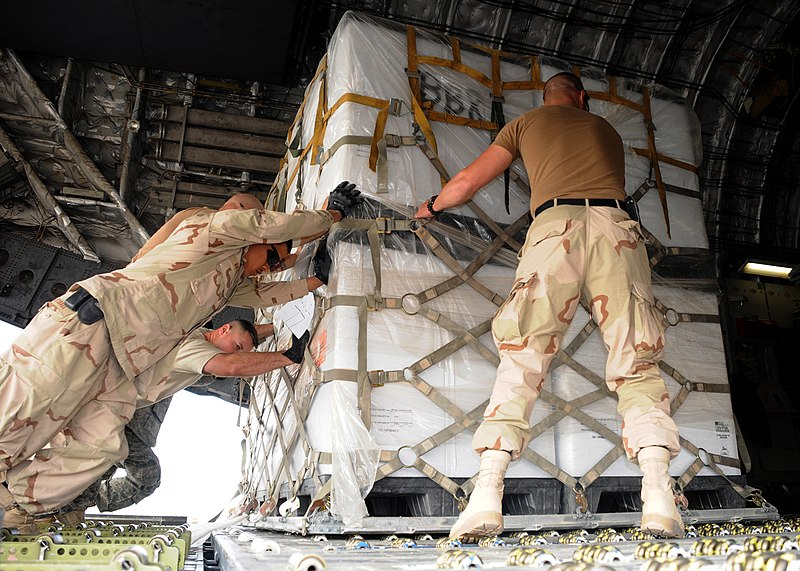
\includegraphics[scale=0.3]{Images/packed.jpg}
	\caption{A packed content on a 463L pallet inside a {\it Boeing C-17}}
	\small\textsuperscript{Source: From Wikimedia Commons, the free media repository}
	\label{fig:larger2}
\end{figure}

Throughout this text, we call {\it packed content}\/ a set of items of same destination stacked on a pallet and covered with a restraining net (see Figure \ref{fig:larger2}). It is considered a single item, having the same attributes of its components, whose values are the sum of individual scores, weights and volumes. To ensure accuracy in pickup and delivery operations, a packed content must remain on board until its destination.


\subsection{Aircraft parameters and load balancing}

We consider real scenarios with an single aircraft with payload of $75,000 kg$, with enough fuel for a range of $4,400km$. The aircraft layout is presented in Figure \ref{fig:larger}, where the pallets positions are identified by $p_i$, $1\leq i \leq 18$.


\begin{figure}[!h]
	\centering
	
	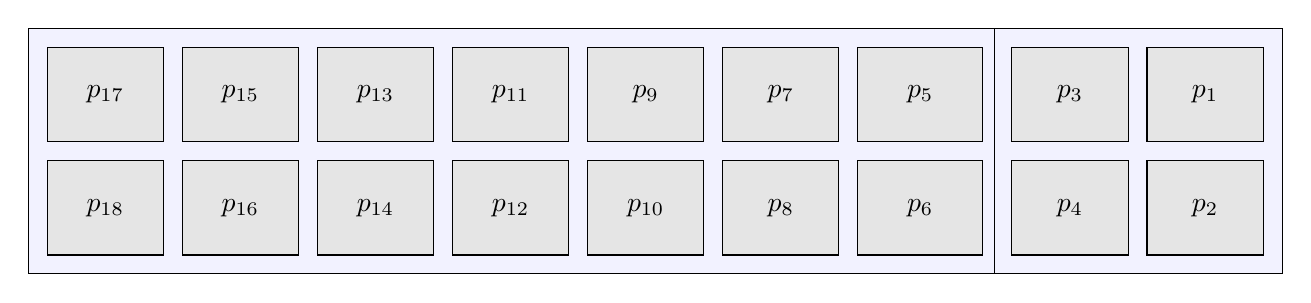
\begin{tikzpicture}[scale=1.2, samples=100]
		
		\filldraw[fill=blue!5!white, draw=black] (0, 0) rectangle (10.23, 2.6);
		
		\filldraw[fill=gray!20!white, draw=black] (0.20, 1.40) rectangle node{$p_{17}$} (1.43, 2.40);
		\filldraw[fill=gray!20!white, draw=black] (0.20, 0.20) rectangle node{$p_{18}$} (1.43, 1.20);
		
		\filldraw[fill=gray!20!white, draw=black] (1.63, 1.40) rectangle node{$p_{15}$} (2.86, 2.40);
		\filldraw[fill=gray!20!white, draw=black] (1.63, 0.20) rectangle node{$p_{16}$} (2.86, 1.20);
		
		\filldraw[fill=gray!20!white, draw=black] (3.06, 1.40) rectangle node{$p_{13}$} (4.29, 2.40);
		\filldraw[fill=gray!20!white, draw=black] (3.06, 0.20) rectangle node{$p_{14}$} (4.29, 1.20);
		
		\filldraw[fill=gray!20!white, draw=black] (4.49, 1.40) rectangle node{$p_{11}$} (5.72, 2.40);
		\filldraw[fill=gray!20!white, draw=black] (4.49, 0.20) rectangle node{$p_{12}$} (5.72, 1.20);
		
		\filldraw[fill=gray!20!white, draw=black] (5.92, 1.40) rectangle node{$p_{9}$} (7.15, 2.40);
		\filldraw[fill=gray!20!white, draw=black] (5.92, 0.20) rectangle node{$p_{10}$} (7.15, 1.20);
		
		\filldraw[fill=gray!20!white, draw=black] (7.35, 1.40) rectangle node{$p_{7}$} (8.58, 2.40);
		\filldraw[fill=gray!20!white, draw=black] (7.35, 0.20) rectangle node{$p_{8}$} (8.58, 1.20);
		
		\filldraw[fill=gray!20!white, draw=black] (8.78, 1.40) rectangle node{$p_{5}$} (10.1, 2.40);
		\filldraw[fill=gray!20!white, draw=black] (8.78, 0.20) rectangle node{$p_{6}$} (10.1, 1.20);
		
		\filldraw[fill=blue!5!white, draw=black] (10.23, 0) rectangle (13.27, 2.6);
		\filldraw[fill=gray!20!white, draw=black] (10.41, 1.40) rectangle node{$p_{3}$} (11.64, 2.40);
		\filldraw[fill=gray!20!white, draw=black] (10.41, 0.20) rectangle node{$p_{4}$} (11.64, 1.20);
		\filldraw[fill=gray!20!white, draw=black] (11.84, 1.40) rectangle node{$p_{1}$} (13.07, 2.40);
		\filldraw[fill=gray!20!white, draw=black] (11.84, 0.20) rectangle node{$p_{2}$} (13.07, 1.20);
		
	\end{tikzpicture}
	
	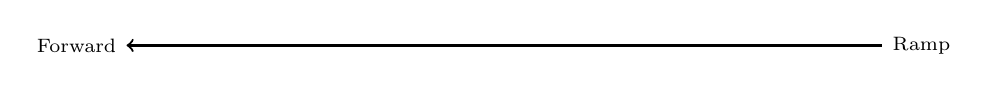
\begin{tikzpicture}[scale=1.2, samples=100]
		\draw[black, thick][<-]  (1, 2.77) node[anchor=east, font=\fontsize{7}{3.5}\selectfont]{Forward} -- (9, 2.77) node[anchor=west, font=\fontsize{7}{3.5}\selectfont]{Ramp} ;
	\end{tikzpicture}
	
	\caption{Aircraft layout} \label{fig:larger}
\end{figure}


The torque applied to the aircraft must keep its CG in the operational range, which corresponds to a fixed percentage of the {\it Mean Aerodynamic Chord} \footnote{Chord is the distance between the leading and trailing edges of the wing, measured parallel to the normal airflow over the wing. The average length of the chord is known as the {\it Mean Aerodynamic Chord} (MAC).} which is considered $1.17m$ for the aircraft of this work (see Figure \ref{fig:lateral}).


\begin{figure}[H]
	\centering
	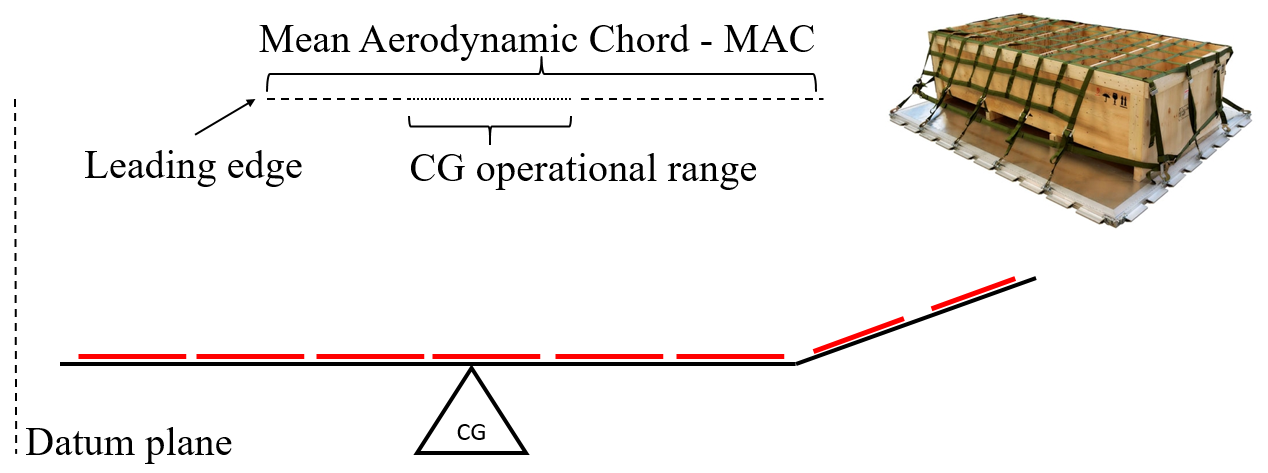
\includegraphics[scale=0.22]{Images/lateral.png}
	\caption{Aircraft longitudinal cut, where red lines are pallets positions}
	\label{fig:lateral}
\end{figure}

Table \ref{tab:larger} shows the parameters of this aircraft. $p_i$\/ are pallets, $1\leq i \leq 18$, with weight $W_i$\/ and $V_i$\/ volume limits, respectively. $D_i^{long}$\/ and $D_i^{lat}$\/ are, respectively, the longitudinal and lateral distances of each pallet centroids to the CG of aircraft along both axes. These distances will be used in the calculation of the torque referring to the items allocated on each pallet. In this aircraft, as the ramp have an inclination of $25^{\circ}$, we made the necessary corrections in $D_i^{long}$, $W_i$\/ and $V_i$\/ of the corresponding pallets.

\begin{table}[H]
	\centering
	\caption{Aircraft parameters}  \label{tab:larger}
	\footnotesize
	\begin{tabular}{c | c c c c c c c c c}
		\toprule
		& \multicolumn{3}{c}{$Payload$: 75,000kg} & \multicolumn{3}{c}{$limit^{CG}_{long}$: $1.170m$} &
		\multicolumn{3}{c}{$limit^{CG}_{lat}$: $0.19m$} \\
		\midrule
		\multirow{2}{*}{{\boldm{$p_i$}}}  & $p_{17}$ & $p_{15}$ & $p_{13}$ & $p_{11}$ & $p_{9}$ & $p_{7}$ & $p_{5}$ & $p_{3}$ & $p_{1}$ \\
		& $p_{18}$ & $p_{16}$ & $p_{14}$ & $p_{12}$ & $p_{10}$ & $p_{8}$ & $p_{6}$ & $p_{4}$ & $p_{2}$ \\
		\midrule 
		\multirow{2}{*}{\boldm{$D_i^{long}$} ($m$)} & -17.57 & -13.17 & -8.77 & -4.40 & 0 & 4.40 & 8.77 & 11.47 & 14.89 \\
		& -17.57 & -13.17 & -8.77 & -4.40 & 0 & 4.40 & 8.77 & 11.47 & 14.89 \\			
		\midrule 
		\multirow{2}{*}{\boldm{$D_i^{lat}$} ($m$)}  & 1.32 & 1.32 & 1.32 & 1.32 & 1.32 & 1.32 & 1.32 & 1.32 & 1.32 \\
		& -1.32 & -1.32 & -1.32 & -1.32 & -1.32 & -1.32 & -1.32 & -1.32 & -1.32 \\	
		\midrule
		{\boldm{$W_i$}} ($kg$)      &   4,500   &    4,500  &   4,500   &  4,500    & 4,500     & 4,500     & 4,500     & 3,000    & 3,000   \\
		{\boldm{$V_i$}} ($m^3$)   &   14.8   &   14.8   &  14.8    &  14.8    & 14.8     & 14.8     & 14.8     & 10.0    & 7.0 \\	
		\midrule	
		
		\textbf{Fuel cost}  & \multicolumn{9}{c}{ $c_d$ = US\$ $4.90/km$ }	 \\
		
		\midrule
		
		\textbf{Fuel consumption rate}  & \multicolumn{9}{c}{ $c_g = 5\%$} \\		
		
		\midrule
		
		\textbf{Maximum weight}  & \multicolumn{9}{c}{ $W_{max} = \sum_i W_i = 75,000kg$} \\
		
		\bottomrule
	\end{tabular}
	\normalsize 
\end{table}


This aircraft spends $c_d$\/ dollars per kilometer flown, and can carry up to $W_{max}$\/ of cargo distributed on the pallets. The {\it fuel consumption rate}\/ $c_g$\/ is the percentage limit of cost increase  due to the CG deviation on the longitudinal axis of the aircraft. $c_g$\/ depends on the characteristics of the aircraft, and is an arbitrated value that should be better evaluated in future research. It is important to consider that the $c_g$\/ tends to zero as the aircraft attitude tends to level. As the CG deviation varies from $0$\/ to $limit^{CG}_{long}$, the {\it fuel cost}\/ increase varies from $0$\/ to $c_g$.


\vspace{3mm}
We also make the following assumptions:
\begin{itemize}
	\item on each pallet, the items are distributed in such a way that their CG coincides with the centroid of the pallet;
	\item the CG of the total load must be at a maximum longitudinal distance $limit^{CG}_{long}$\/ from the CG of the aircraft;
	\item the CG of the total load must be at a maximum lateral distance $limit^{CG}_{lat}$\/ from the CG of the aircraft;
	\item the pallets are distributed in two identical rows (with odd and even indices, respectively), and the centroid of $p_i$\/ is at distance $D^{lat}_{i}$\/ from the center-line of the aircraft.
\end{itemize}



\section{The mathematical modeling}
\label{sec4}

Given the assumptions and parameters described in the previous section, we are ready to present the mathematical modeling of ACLP+RPDP. 

ACLP+RPDP has the objective function \ref{eq1}, and the calculus equations \ref{eq:scores} to \ref{eq:LatPacked} subject to constraints \ref{eq:torqlat} to \ref{eq21}, which will be described below. 

\subsection{Problem structure and input data}

In the definitions below and in the tests of Section \ref{sec6}, we use the values assigned in Tables \ref{tab:costs} and \ref{tab:larger}. To simplify the notation throughout this text, $p_i$\/ will be called pallet $i$, and $l_k$\/ will be called node $k$.

Let $L = \{ 0, 1, \ldots, K \}$ be the set with the $K+1$\/ nodes, and let $L_k$\/ be the set of remaining nodes when the aircraft is in the node $k$, $0 \leq k \leq K$. Therefore, $L_0 = L$.

Let $d(a,b)$ be the distance from node $a$\/ to node $b$, where $0 \leq a, b \leq K$. By definition, $d(a,a) = 0, \forall a$.

Let $C=\left[c_{a,b}\right]$\/ be the cost matrix of flights, where $c_{a,b} = c_d*d(a,b), 0 \leq a,b \leq K$.

Let $M = \{1, 2, \ldots, m \}$\/ the set of $m$\/ empty pallets assigned to specific positions within the aircraft. In Table \ref{tab:larger}, $m=18$. Each pallet $i$, $1 \leq i \leq m$, has weight capacity $W_i$, volume capacity $V_i$, longitudinal distance to the CG of aircraft $D^{long}_i$, and lateral distance to the center line of aircraft $D^{lat}_i$. 

Let $N_k = \{1, \ldots, n_k \}$\/ be the set of $n_k$\/ items $t_j^k$\/ available for loading on the node $k$, $1 \leq j \leq n_k$, $0 \leq k \leq K$. For ease of notation, $t_j^k$\/ will be called item $j$\/ of the node $k$, with score $s_j$, weight $w_j$, volume $v_j$, and destination $to_j \in L_k$. Let $N = \bigcup_{0 \leq k \leq K} N_k$ be the set of items of all nodes along a tour.

Let $Q_k = \{1, \ldots, m_k \}$\/ be the set of $m_k \leq m$\/ packed contents $a^k_q$\/ at the node $k$, $1 \leq q \leq m_k$, $0 \leq k \leq K$. For ease of notation, $a^k_q$\/ will be called packed content $q$\/ of the node $k$, with total weight $w_q$, total volume $v_q$, and destination $to_q \in L_k$. By definition, $m_0 = 0$, and therefore $Q_0 = \varnothing$. Packed contents that were destined to node $k$\/ are unloaded when the aircraft arrives at this node, that is, they are not considered in $Q_k$.


\subsection{The decision variables}

Let $X_{ij}^k$\/ and $Y_{iq}^k$\/ be binary variables, where $1 \leq i \leq m$, $1 \leq j \leq n_k$, $1 \leq q \leq m_k$\/ and $0 \leq k \leq K$.

$X_{ij}^k = 1$\/ if the item $j$\/ of the node $k$\/ is assigned to the pallet $i$, and 0 otherwise.

$Y_{iq}^k = 1$\/ if the packed content $q$\/ of the node $k$\/ is assigned to the pallet $i$, and 0 otherwise.


\subsection{The allocation graph}

Allocations of items or packed contents to the pallets in the node $k$\/ can be seen as a bipartite graph $G_k(V_k, E_k)$, where:

\begin{itemize}

\item $V_k = M \cup N_k \cup Q_k$;

\item $E_k = E_{N_k} \cup E_{Q_k}$;

\item $(i, j) \in E_{N_k}$\/ if $X_{ij}^k = 1$, where $i$\/ is a pallet and $j$\/ is a item of the node $k$;

\item $(i, q) \in E_{Q_k}$\/ if $Y_{iq}^k = 1$, where $i$\/ is a pallet and $q$\/ is a packed content of the node $k$.

\end{itemize}

\subsection{The objective function}

Let $S_K = \{s: \{1, \dots, K\} \rightarrow \{1, \dots, K\} \}$\/ be the set of $K!$ permutations $\pi$, which correspond to all possible tours (or itineraries) that have node $0$\/ as origin and end, passing through the other $K$\/ nodes. Let $\pi_k$\/ be $k^{th}$\/ node of the tour $\pi$, $1 \leq k \leq K$. In this way, the tour $\pi$\/ is described as $\{0,\pi_1,\ldots,\pi_K, 0\}$. For ease of notation, we can define $\pi_0 = \pi_{K+1} = 0$.

The objective of ACLP+RPDP is to find the permutation $\pi \in S_K$, with the corresponding allocation of items on the pallets at each node, that maximizes the function $f_\pi = \tilde{s}_\pi/\tilde{c}_\pi$ \ref{eq1}, where $\tilde{s}_\pi$\/ is the total score of transported items, and $\tilde{c}_\pi$\/ is the total cost of fuel consumed. 

\begin{equation} \label{eq1}
	\max_{\pi \in S_K} f_\pi = \tilde{s}_\pi/\tilde{c}_\pi
\end{equation}



\subsection{The calculus equations}


We have the following calculation equations:

\begin{itemize}
	\item $\tilde{s}_\pi$\/ \ref{eq:scores} is the sum of the scores of the items loaded on the aircraft throughout the tour $\pi$.
	\item $\tau_{\pi_k}$\/ \ref{eq:tau} is the longitudinal torque applied by the loaded pallets at the node ${\pi_k}$, in proportion relative to the highest torque supported by the aircraft.
	\item $\tilde{c}_\pi$\/ \ref{eq:costs} is the cost of to the total fuel consumed in the tour $\pi$\/ due to the distances traveled and the CG longitudinal deviations \footnote{In our experiments, we found that the magnitude of the lateral torque was always very small, and therefore we decided to ignore it in the fuel consumption.} in each pallet.
	\item The sets of nodes not yet visited along the tour $\pi$\/ are defined in \ref{eq:pdp11} and \ref{eq:departing}.
	\item At the beginning of the tour $\pi$, there are no packed contents \ref{eq:pdp13}. 
	\item $\epsilon_{\pi_k}^t$\/ \ref{eq:LatItem} and $\epsilon_{\pi_k}^a$\/ \ref{eq:LatPacked} are the lateral torque applied by the loaded pallets at the node ${\pi_k}$, in proportion relative to the highest torque supported by the aircraft. For ease of notation, $\epsilon_{\pi_k}^t$\/ corresponds to the items, and $\epsilon_{\pi_k}^a$\/ to the packed contents.
\end{itemize}

\begin{equation} \label{eq:scores}
	\tilde{s}_\pi = \sum_{k=0}^{K} \sum_{i=1}^{m} \sum_{j=1}^{n_{\pi_k}} X_{ij}^{\pi_k} \times s_j
\end{equation}


\begin{equation} \label{eq:tau}
	\tau_{\pi_k} = \sum_{i=1}^{m} \Big [ D_i^{long} \times \Big ( \sum_{j=1}^{n_{\pi_k}} X_{ij}^{\pi_k} \times w_j +  \sum_{q=1}^{m_{\pi_k}} Y_{iq}^{\pi_k} \times w_q \Big ) \Big ] \Big / W_{max} \times limit^{CG}_{long}; \ k \in \{0, \ldots, K\}
\end{equation}


\begin{equation} \label{eq:costs}
	\tilde{c}_{\pi} = \sum_{k=0}^{K} \Big [ c_{\pi_k, \pi_{k+1}}\times(1+c_g\times|\tau_{\pi_k}|) \Big ] 
\end{equation}



\begin{equation} \label{eq:pdp11}
	L_0 = L
\end{equation}

\begin{equation} \label{eq:departing}
	L_{\pi_k} = L_{\pi_{k-1}} - \{\pi_k\}; \ k \in \{1, \ldots, K\}
\end{equation}


	
\begin{equation} \label{eq:pdp13}
	m_0 = 0
\end{equation}


\begin{equation} \label{eq:LatItem}
	\epsilon_{\pi_k}^t = \sum_{i=1}^{m} \Big [ D_i^{lat} \times \sum_{j=1}^{n_{\pi_k}} \Big ( X_{ij}^{\pi_k} \times w_j \times (i\%2) - X_{ij}^{\pi_k} \times w_j \times (i+1)\%2 \Big ) \Big ] \Big / W_{max} \times limit^{CG}_{lat}; \ k \in \{0, \ldots, K\}
\end{equation}

\begin{equation} \label{eq:LatPacked}
	\epsilon_{\pi_k}^a = \sum_{i=1}^{m} \Big [ D_i^{lat} \times \sum_{q=1}^{m_{\pi_k}} \Big ( Y_{iq}^{\pi_k} \times w_q \times (i\%2) - Y_{iq}^{\pi_k} \times w_q \times (i+1)\%2 \Big ) \Big ] \Big / W_{max} \times limit^{CG}_{lat}; \ k \in \{0, \ldots, K\}
\end{equation}



\subsection{The constraints}

Finally, we can consider the constraints at each node $\pi_k$:

\begin{itemize}
	\item The longitudinal \ref{eq:torqlong} and the lateral \ref{eq:torqlat} torques must be within the limits of the aircraft.
	\item The items allocated to each pallet cannot exceed its weight \ref{eq:app2} and volume \ref{eq:app3} limits.
	\item At most, each item is associated with a single pallet \ref{eq:app4};
	\item Packed contents that have not yet reached their destination must remain on board \ref{eq:app5}.
	\item Items allocated on the same pallet must have the same destinations. In this case, we need two constraints: \ref{eq18} and \ref{eq19}. If $X_{ia}^{\pi_k} = X_{ib}^{\pi_k} = 1$, both constraints require that $to_a = to_b$; otherwise these constraints have no effect.
	\item If there is a packed content on the pallet, it must also have the same destination as the other items. Similarly, we use two constraints: \ref{eq20} and \ref{eq21}.
\end{itemize}


\begin{equation} \label{eq:torqlong}
	| \tau_{\pi_k} | \leq 1;\ k \in \{0, \ldots, K\}
\end{equation}

\begin{equation} \label{eq:torqlat}
	| \epsilon_{\pi_k}^t + \epsilon_{\pi_k}^a| \leq  1; \ k \in \{0, \ldots, K\}
\end{equation}

\begin{equation} \label{eq:app2}
	\sum_{j=1}^{n_{\pi_k}} X_{ij}^{\pi_k} \times w_j + \sum_{q=1}^{m_{\pi_k}} Y_{iq}^{\pi_k} \times w_q  \leq W_i; \ i \in \{1, \ldots, m\}; \ k \in \{0, \ldots, K\}
\end{equation}

\begin{equation} \label{eq:app3}
	\sum_{j=1}^{n_{\pi_k}} X_{ij}^{\pi_k} \times v_j + \sum_{q=1}^{m_{\pi_k}} Y_{iq}^{\pi_k} \times v_q  \leq\ V_i; \ i \in \{1, \ldots, m\}; \ k \in \{0, \ldots, K\}
\end{equation}

\begin{equation} \label{eq:app4}
	\sum_{i=1}^{m} X_{ij}^{\pi_k} \leq 1; \ j \in \{1, \ldots, n_{\pi_k}\}; \ k \in \{0, \ldots, K\}
\end{equation}

\begin{equation} \label{eq:app5}
	\sum_{i=1}^{m} Y_{iq}^{\pi_k} = 1;\ to_q \in L_{\pi_k}; \ q \in \{1, \ldots, m_{\pi_k}\}; \ k \in \{0, \ldots, K\}
\end{equation}

\begin{equation} \label{eq18}
	to_a - to_b \geq -K \times (1-X_{ia}^{\pi_k} \times X_{ib}^{\pi_k}); \ i \in \{1, \ldots, m\}; \ a,b \in \{1, \ldots, n_{\pi_k}\}; \ k \in \{0, \ldots, K\}
\end{equation}

\begin{equation} \label{eq19}
	to_a - to_b \leq K \times (1-X_{ia}^{\pi_k} \times X_{ib}^{\pi_k}); \ i \in \{1, \ldots, m\}; \ a,b \in \{1, \ldots, n_{\pi_k}\}; \ k \in \{0, \ldots, K\}
\end{equation}

\begin{equation} \label{eq20}
	to_j - to_q \geq -K \times (1-X_{ij}^{\pi_k} \times Y_{iq}^{\pi_k}); \ i \in \{1, \ldots, m\}; \ j \in \{1, \ldots, n_{\pi_k}\}; \ q \in \{1, \ldots, m_{\pi_k}\}; \ k \in \{0, \ldots, K\}
\end{equation}

\begin{equation} \label{eq21}
	to_j - to_q \leq  K \times (1-X_{ij}^{\pi_k} \times Y_{iq}^{\pi_k}); \ i \in \{1, \ldots, m\}; \ j \in \{1, \ldots, n_{\pi_k}\}; \ q \in \{1, \ldots, m_{\pi_k}\}; \ k \in \{0, \ldots, K\}
\end{equation}

Constraints \ref{eq18} to \ref{eq21} are not within standard {\it Mixed-Integer Programming}\/ (MIP), and therefore need to be handled in a different way. In the next section, we will explain the strategy adopted to solve ACLP+RPDP.


\section{Solution strategy}
\label{sec5}

Once the assumptions of this work and the mathematical modeling of the problem are presented, it is possible to see that ACLP+RPDP is {\it NP-hard}.

 {\color{red}  In a similar way to Lurkin and Schyns \cite[p. 6]{LurkinSchyns2015}, consider the simple case where $K=1$\/ (one leg), $m=2$\/ (two pallets around the aircraft CG), $2n$\/ sufficiently light items with same scores in node 0, and no items in node 1. Under these conditions, through polynomial reductions for the {\it Set-Partition Problem}, it is possible to demonstrate that the decision problem associated with ACLP+RPDP is {\it NP-complete}.}

Throughout our research, we have thoughtfully described the ACLP+RPDP model in standard MIP format and found that no MIP solver can handle its practical cases in a feasible time. Thus, as ACLP+RPDP is highly complex, involving four intractable subproblems (APP, WBP, PDP and TSP), our strategy will be to focus only on {\it real cases}\/ and to develop quick node-by-node solutions, not necessarily optimal, that allow to build a complete tour.

The ACLP+RPDP solution defines a tour and a corresponding loading and unloading plan at each node. In this way, the loading and unloading time will be limited only by the use of the equipment at each node. Therefore, there will only be waiting time at the base node, corresponding to the runtime of ACLP+RPDP algorithm. For this reason, our method will also be parameterized by the maximum time that can be waited until the start of the load in the base node.

On the other hand, we know that transport aircraft generally have a few dozen pallets, the flight plan has less than $6$\/ nodes, and each node has hundreds of items to be shipped. We also know that missions with fewer nodes are more frequent than longer missions. Under these circumstances, we can adopt two more strategies:

\begin{itemize}
	
\item We will consider that the number of destinations is greater than 1, to avoid the case of a single and trivial tour, but less than the number of pallets, that is, $1 < K < m$. So we can preset the destinations of the pallets at each node. In this way, we will reserve a number of pallets proportional to the volume demanded by each destination at the shipping node. We could have used another criterion, but it was observed in the experiments that volume is more constrictive in airlift.
	
\item If we have quick node-by-node solutions, as the number of nodes is small we have the possibility to check the solution corresponding to the tour with the shortest total distance, and even test all possible tours, selecting the one that provides the best value for the objective function.


\end{itemize}

Our complete strategy is summarized in Algorithm \ref{alg:main}.

\begin{algorithm}[H]
	\caption{Solving ACLP+RPDP}  \label{alg:main}
	\begin{algorithmic}[1]
		
		\Procedure{$ACLP+RPDP$}{$scenario, surplus, tmax$}

		\State Let aircraft and $M$  \label{main:M} \Comment{Aircraft parameters from Table \ref{tab:larger}}
		
		\State Let $K$, $L$\/ and $C$ be according to $scenario$ \label{main:KLC} \Comment{Nodes and costs from Tables \ref{tab:costs} and \ref{tab:scenarios}}
		
		\State Let $\pi_{TSP1}$\/ and $\pi_{TSP2}$  \Comment{The shortest tours from Tables \ref{tab:costs} and \ref{tab:scenarios}}
		
		\State $N \gets ItemsGeneration(scenario, surplus)$ \label{main:items} \Comment{Items available for shipment}
		
		\For {each $method$} \Comment{$method$ is a MIP solver or a heuristic}
		
			\State $f_1 \gets SolveTour(\pi_{TSP1}, L, M, C, N, method, tmax)$  \label{main:f1} 

		    \State $f_2 \gets SolveTour(\pi_{TSP2}, L, M, C, N, method, tmax)$  \label{main:f2}
		
			\State $answer1[scenario,surplus,method] \gets max( f_1, f_2  )$  \label{main:a1} \Comment{Best result between the shortest tours}
			
			\For {each $\pi \in S_K$} \label{main:loop1} \Comment{$\pi$ is a permutation of nodes (a tour)}
			
				\State $f_{\pi} \gets SolveTour(\pi, L, M, C, N, method, tmax/K!)$ \Comment{$f_{\pi}$\/ is a solution to the tour $\pi$} \label{main:fpi}
				
			\EndFor \label{main:loop2}
			\State $answer2[scenario,surplus,method] \gets \max f_{\pi}$ \label{main:a2} \Comment{Best result among all permutations}
		\EndFor
		
		\Return $answer1, answer2$
		
		\EndProcedure
		
	\end{algorithmic}
\end{algorithm}


The aircraft parameters and the set $M$\/ of pallets are in Table \ref{tab:larger}. In this algorithm, we use five values for $scenario$, according to Tables \ref{tab:costs} and \ref{tab:scenarios}, which define the number $K$ of destinations, the set $L$\/ of nodes, the costs $C$\/, and the shortest tours $\pi_{TSP1}$\/ and $\pi_{TSP2}$.

\vspace{2.0mm}
\begin{table}[H]
	\centering
	\caption{Testing scenarios}  \label{tab:scenarios}
	\begin{tabular}{c c c c c}
		\toprule
		{\bf Scenario} & $K$ & $L$ & $\pi_{TSP1}$ & $\pi_{TSP2}$ \\		
		\midrule
		1 & 2    & \{$0,1,2$\}           & 0 1 2 0  & 0 2 1 0 \\
		2 & 3    & \{$0,1,2,3$\}         & 0 1 2 3 0 & 0 3 2 1 0\\
		3 & 4    & \{$0,1,2,3,4$\}       & 0 4 1 2 3 0 & 0 3 2 1 4 0 \\
		4 & 5    & \{$0,1,2,3,4,5$\}     & 0 4 1 2 5 3 0 & 0 3 5 2 1 4 0 \\
		5 & 6    & \{$0,1,2,3,4,5,6$\}   & 0 4 1 2 6 5 3 0 & 0 3 5 6 2 1 4 0 \\
		\bottomrule
	\end{tabular}
\end{table}

$surplus$\/ is a value in $\{1.2, 1.5, 2.0\}$, which corresponds, at each node $k$, to the ratio between the sum of the volumes of the items  and the load capacity of the pallets ($surplus = \sum_{j=1}^{n_k} v_j$/$\sum_{i=1}^{m} V_i$). This parameter allows us to verify the different behavior of each $method$, according to $scenario$\/ and the quantity of items available for shipment. It is passed to $ItemsGeneration$\/ (line \ref{main:items}), responsible for creating the items to be shipped, which will be presented in the next section (Algorithm \ref{alg:itemsgen}).

$tmax$\/ is a runtime limit, which will be distributed among the tours (lines \ref{main:f1}, \ref{main:f2} and \ref{main:fpi}). $method$\/ corresponds to a MIP solver or a heuristic to the node-by-node solution $SolveTour$, which will be presented in subsection \ref{methods}.

The best results corresponding to the shortest tours are stored in $answer1$\/ (line \ref{main:a1}), and those obtained by testing all $K!$\/ tours are stored in $answer2$\/ (line \ref{main:a2}).

Next, we will present two subsections: in the first we explain how $SolveTour$\/ is executed, presetting the destinations of the pallets. In the second we will present the heuristics developed for node-by-node solutions.


\subsection{SolveTour algorithm}
\label{tour}


As we commented in the previous subsection, we will adopt the strategy of presetting the destinations of each pallet throughout the tour. This is feasible in practical cases, where $1<K<m$. For this, each pallet $i$\/ also has a field $T^k_i$, $0\leq k \leq K$, which stores its next destination after being loaded at node $k$. For this reason, $T^k_i \in L_k$, $1 \leq i \leq m$, $0\leq k \leq K$.


$SolveTour$\/ is described in Algorithm \ref{alg:tour}, where $\pi$\/ is a permutation of the nodes (excluding the base) that defines the order of visits in this tour, $method$\/ corresponds to a MIP solver or a heuristic for solving the node-by-node problems, and $tmax$\/ is the runtime limit that will be distributed among the $K+1$\/ legs of the tour.


\begin{algorithm}[H]
	\caption{Solving the tour $\pi$ with $method$}  \label{alg:tour}
	\begin{algorithmic}[1]
		
		\Procedure{$SolveTour$}{$\pi, L, M, C, N, method$, $tmax$}
		
		\State $\pi_0     \gets 0$ \label{tour:pi1} \Comment{Base $0$\/ is the first node}
		\State $\pi_{K+1} \gets 0$ \label{tour:pi2} \Comment{Base $0$\/ is the last node}
		
		\State $score \gets 0$ \label{tour:score}
		\State $cost  \gets 0$ \label{tour:cost}
		
		\For {$k \gets 0$ to $K$} \label{tour:loop1}	
		\State $L_{\pi_k} \gets L - \{\pi_0,\pi_1,\ldots,\pi_k\}$  \label{tour:lk1}	\Comment{$\pi_k$ is the current node}	
		\State $T_i^{\pi_k} \gets -1$, $1 \leq i \leq m$ \label{tour:-1} \Comment{Unset the pallet destinations}

		\If {$k = 0$}
		\State Let $G_1(M \cup N_0, \varnothing)$ \label{tour:g11}
		\Else
	
		\State $E_{Q_{\pi_k}}, M \gets UpdatePacked(M, Q_{\pi_k}, \pi_k)$ \label{tour:dest}			
		\State Let $G_1(M \cup N_{\pi_k} \cup Q_{\pi_k}, E_{Q_{\pi_k}})$ \label{tour:g12}
		\EndIf  \label{tour:lk2}	
		
		\State $M \gets SetPalletsDestinations(M, \pi_k )$ \label{tour:dest2}
		
		\State $G_2 \gets SolveNode(method, \pi_k, G_1, tmax/(K+1))$ \Comment{Each tour has $K+1$\/ legs} \label{tour:node}
		
		\State $s, \tau \gets ScoreAndDeviation(\pi_k, G_2)$ \label{tour:analyse}
		
		\State $score \gets score + s$ \label{tour:score2}
		\State $cost  \gets cost  + c_{\pi_k,\pi_{k+1}} \times (1 + c_g \times |\tau|)$ \label{tour:cost2} 
		
		\EndFor  \label{tour:loop2}
		
		\Return $score / cost$ \label{tour:f}
		
		\EndProcedure
		
	\end{algorithmic}
\end{algorithm}


As we mentioned in the previous section, all tours start and end at the base $0$\/ (lines \ref{tour:pi1}-\ref{tour:pi2}). After initializing the score and cost values (lines \ref{tour:score}-\ref{tour:cost}), there is a loop for the $K+1$\/ flights (lines \ref{tour:loop1}-\ref{tour:loop2}). Initially, the set $L_{\pi_k}$\/ of remaining nodes is updated (line \ref{tour:lk1}), and the pallet destinations are unset (line \ref{tour:-1}).

When the aircraft is at the base, the initial graph $G_1$\/ is empty and there is no packed contents \ref{tour:g11}. Otherwise, $UpdatePacked$\/ (line \ref{tour:dest}) returns the set of packed contents that have not yet reached their destination and remain on board, rearranging them on the pallets to minimize CG deviation. This allocation is stored in graph $G_1$\/ (line \ref{tour:g12}).

$SetPalletsDestinations$\/ (line \ref{tour:dest2}) presets the destination of each pallet based on the volume demands of the current node, without changing the pallets destination with packed contents.

Finally, $SolveNode$\/ includes the edges corresponding to the items shipped at the current node, returning the graph $G_2$\/ (line \ref{tour:node}). The score and the CG deviation of $G_2$\/ are calculated (line \ref{tour:analyse}) and accumulated (lines \ref{tour:score2}-\ref{tour:cost2}), allowing the final result of this tour (line \ref{tour:f}).


$UpdatePacked$, described in Algorithm \ref{alg:cons}, finds the best packed-pallet allocation, in terms of CG deviation, for the packed contents that remain on board. 


\begin{algorithm}[H]
	\caption{Updating the packed contents that remain boarded at the node $\pi_k$}  \label{alg:cons}
	\begin{algorithmic}[1]
		
		\Procedure{$UpdatePacked$}{${M, Q_{\pi_k}, \pi_k}$}
		
		\State $E_{Q_{\pi_k}} \gets MinCGDeviation(E_{Q_{\pi_k}})$ \Comment{Using a MIP solver} \label{cons:minCG}
		
		\For{$i \gets 1$ to $m$} \label{cons:Ybegin}
		
		\For{$q \gets 1$ to $m_{\pi_k}$}
		
		\State $T_i^{\pi_k} \gets -1$
		
		\If{$(i, q) \in E_{Q_{\pi_k}}$} 
		\State $T_i^{\pi_k} \gets to_q$   \Comment{Set the pallet destinations}
		\EndIf
		\EndFor		
		\EndFor \label{cons:Yend}
		
		\Return $E_{Q_{\pi_k}}, M$
		
		\EndProcedure
		
	\end{algorithmic}
\end{algorithm}

$MinCGDeviation$\/ (line \ref{cons:minCG}) relocates the packed contents on the pallets, minimizing torque and ensuring that they all remain on board, one packed content on each pallet. It is run through a MIP solver with objective function \ref{eq:torque} and constraints \ref{eq:embarked} and \ref{eq:one}. As there are few variables, $E_{Q_{\pi_k}}$\/ is obtained in less than $30$\/ milliseconds. Finally, the destination of each pallet with a packed content is updated (lines \ref{cons:Ybegin}-\ref{cons:Yend}).

\begin{equation} \label{eq:torque}
	\min f =  \Big | \sum_{i=1}^{m} \sum_{q=1}^{m_{\pi_k}} Y^k_{iq} \times w_q \times D_i^{long}  \Big |
\end{equation}

\begin{equation} \label{eq:embarked}
	\sum_{i=1}^{m} Y^k_{iq} = 1;\ q \in \{1,\ldots,m_{\pi_k}\}
\end{equation}

\begin{equation} \label{eq:one}
	\sum_{q=1}^{m_{\pi_k}} Y^k_{iq} \leq 1;\ i \in \{1,\ldots,m\}
\end{equation}


$SetPalletsDestinations$, which sets the pallets destination not yet defined, is described in Algorithm \ref{alg:dest}.



\begin{algorithm}[H]
	\caption{Setting pallets destination based on the items to be embarked at the node $\pi_k$}  \label{alg:dest}
	\begin{algorithmic}[1]
		
		\Procedure{$SetPalletsDestinations$}{$M, \pi_k$}
		
			\State $vol_x \gets  0$, $x \in L_{\pi_k}$  \label{dest:vector1}

			\State $max \gets 0$ 
	
			\State $total \gets 0$ 
	
			\For{$j \gets 1$ to $n_{\pi_k}$}
						
				\If {$to_j \in L_{\pi_k}$} 
				
					\State $vol_{to_j} \gets vol_{to_j} + v_j$ 
					\State $total \gets total + v_j$ 
					
					\If {$vol_{to_j} > vol_{max}$}
					
						\State $max \gets to_j$ \label{dest:max} \Comment{$max$\/ is the destination with maximum volume demand}
					\EndIf
					
				\EndIf
				
			\EndFor
					
			\For{$x \in L_{\pi_k}$} \label{dest:propor1}
			
				\If {$vol_{x} \neq 0$}
				
					\State $needed \gets \max \{1, \lfloor{ (m-m_{\pi_k}) \times vol_{x}/total}\rfloor \}$  \Comment{Number of pallets to node $x$}
					
					\State $np \gets 0$
					
					\For{$i \gets 1$ to $m$}
											
						\If{($np < needed$) {\bf and} ($T_i^{\pi_k} = -1$)}
							\State $T_i^{\pi_k} \gets x$
							\State $np \gets np + 1$
						\EndIf
					
					\EndFor
				\EndIf 
				
			\EndFor \label{dest:propor2}
		
			\For{$i \gets 1$ to $m$} \label{dest:max1}
				\If{$T_i^{\pi_k} \gets -1$}  \Comment{Remaining pallets}
					\State $T_i^{\pi_k} \gets max$
				\EndIf
			\EndFor \label{dest:max2}
			
			\Return $M$
			
		\EndProcedure
		
	\end{algorithmic}
\end{algorithm}


$vol$\/ stores the demand volume of items destined to the non-visited nodes (line \ref{dest:vector1}). The destination of empty pallets is defined proportionally to the volume of items to be embarked (lines \ref{dest:propor1}-\ref{dest:propor2}). The destination with the maximum volume defines any remaining pallets (lines \ref{dest:max1}-\ref{dest:max2}).


$ScoreAndDeviation$, described in Algorithm \ref{alg:eval}, evaluates the allocation graph $G$\/ generated by $SolveNode$\/ at node $\pi_k$\/ and returns the corresponding score and CG deviation.


\begin{algorithm}[H]
	\caption{Calculating the score and the relative torque deviation of the graph $G$\/ at the node $\pi_k$}  \label{alg:eval}
	\begin{algorithmic}[1]
		
		\Procedure{$ScoreAndDeviation$}{$\pi_k, G$}
		
		\State Let $G(V_{\pi_k}, E_{Q_{\pi_k}} \cup E_{N_{\pi_k}})$
		
		\State $s \gets 0$
		\State $\tau_i \gets 0$, $1 \leq i \leq m$
		\For{$i \gets 1$ to $m$}	\label{eval:loop1}
						
			\For{$j \gets 1$ to $n_{\pi_k}$}
			
				\If{$X_{ij}^{\pi_k} = 1$}
					\State $s \gets s + s_j$ \label{eval:score1}
					\State $\tau_i \gets \tau_i + w_j \times D_i^{long}$ \label{eval:eps1}
				\EndIf
			\EndFor	
					
			\For{$q \gets 1$ to $m_{\pi_k}$}
				\If{$Y_{iq}^{\pi_k} = 1$}
					\State $s \gets s + s_q$   \label{eval:score2}
					\State $\tau_i \gets \tau_i + w_q \times D_i^{long}$  \label{eval:eps2}
				\EndIf
			\EndFor	   \label{eval:loop2}
		\EndFor
		
		\State $\tau \gets  \sum_{i=1}^{m} \tau_i / (W_{max} \times limit^{CG}_{long})$ \label{eval:torque}
		
		\Return $s,\ \tau$
		\EndProcedure
		
	\end{algorithmic}
\end{algorithm}


This algorithm consists of a loop that goes through all the pallets (lines \ref{eval:loop1}-\ref{eval:loop2}), accumulating the scores (lines \ref{eval:score1} and \ref{eval:score2}) and the torques (lines \ref{eval:eps1} and \ref{eval:eps2}) of the shipped items, allowing the final calculation of the CG deviation (line \ref{eval:torque}).

\subsection{Node-by-node solutions}
\label{methods}


In this subsection we present two implementations of $SolveNode$\/ algorithm: with a MIP solver and a heuristic.


\subsubsection{With a MIP solver}
\label{solver}

Our strategy adopted in $SolveTour$\/ previously defines the values of some variables: the set of nodes to be visited is updated, the packed contents that remain on board are reallocated to minimize the CG deviation, and the pallets destinations are determined according to the volume of items available for shipment. 

In this way, the mathematical modeling for $SolveNode(MIP,\pi_k,G, tmax)$\/ becomes simpler, which finds an allocation of available items at the node $\pi_k$\/ using previously defined values of $L_{\pi_k}$, $T_i^{\pi_k}$, and $a^{\pi_k}_q$. Thus, we use a MIP solver with runtime limit $tmax$\/ at the node $\pi_k$\/ to maximize the objective function \ref{eq:obj2}, with the calculus equations \ref{eq:newf} to \ref{eq:costs2}, subject to the constraints \ref{eq:tau2} to \ref{eq:ifB}. The binary variables $X_{ij}$\/ and $Y_{iq}$\/ define the sets of edges $E_{N_{\pi_k}}$\/ and $E_{Q_{\pi_k}}$, respectively, included in the graph $G$.

\begin{equation} \label{eq:obj2}
	\max f= \tilde{s} / \tilde{c}
\end{equation}

\begin{equation} \label{eq:newf}
	\tilde{s} = \sum_{i=1}^{m} \sum_{j=1}^{n_{\pi_k}} X_{ij} \times s_j
\end{equation}

\begin{equation} 
	\tau_{\pi_k} = \sum_{i=1}^{m} \Big [ D_i^{long} \times (\sum_{j=1}^{n_{\pi_k}} X_{ij} \times w_j +  \sum_{q=1}^{m_{\pi_k}} Y_{iq} \times w_q) \Big ] \Big / W_{max} \times limit^{CG}_{long}
\end{equation}

\begin{equation} \label{eq:costs2}
	\tilde{c} =  c_{\pi_k, \pi_{k+1}}\times(1+c_g\times|\tau_{\pi_k}|)
\end{equation}

\begin{equation} \label{eq:tau2}
	|\tau_{\pi_k}| \leq 1
\end{equation}

\begin{equation} 
	\sum_{j=1}^{n_{\pi_k}} X_{ij} \times w_j + \sum_{q=1}^{m_{\pi_k}} Y_{iq} \times w_q  \leq W_i; \ i \in \{1, \ldots, m\}
\end{equation}

\begin{equation} 
	\sum_{j=1}^{n_{\pi_k}} X_{ij} \times v_j + \sum_{q=1}^{m_{\pi_k}} Y_{iq} \times v_q  \leq\ V_i; \ i \in \{1, \ldots, m\}
\end{equation}

\begin{equation} 
	\sum_{i=1}^{m} X_{ij} \leq 1; \ j \in \{1, \ldots, n_{\pi_k}\}
\end{equation}

\begin{equation} \label{eq:if2}
	X_{ij} = 0;\ to_j \notin L_{\pi_k}; \ i \in \{1, \ldots, m\}; \ j \in \{1, \ldots, n_{\pi_k}\}
\end{equation}

\begin{equation} \label{eq:ifA}
	X_{ij} \leq X_{ij} \times (T_i^{\pi_k} - to_j + 1); \ i \in \{1, \ldots, m\}; \ j \in \{1, \ldots, n_{\pi_k}\}
\end{equation}

\begin{equation} \label{eq:ifB}
	X_{ij} \leq X_{ij} \times (to_j - T_i^{\pi_k} + 1 ); \ i \in \{1, \ldots, m\}; \ j \in \{1, \ldots, n_{\pi_k}\}
\end{equation}

The constraints \ref{eq:ifA} and \ref{eq:ifB} are equivalent to $X_{ij} =1$\/ if $to_j = T_i^{\pi_k}$, and $X_{ij} =0$\/ otherwise .


\subsubsection{With the Shims heuristic}

One of the main objectives of this work was to find a quick heuristic that offers a good-quality solution for the node-by-node problem. Taking this into account, we design algorithms based on known meta-heuristics: {\it Ant Colony Optimization} (ACO) \cite{Dorigo1992, DorigoManiezzoColorni1996}, {\it Noising Method Optimization} (NMO) \cite{CharonHudry1993,CharonHudry2001,Zhan2020}, {\it Tabu Search} (TS) \cite{Glover1986} and {\it Greedy Randomized Adaptive Search Procedure} (GRASP) \cite{FeoResende1989}. We considered several ideas from the literature \cite{NiarFreville1997,Fidanova2006,Laabadi2018,Alonso2019,Zhan2020}, and we were careful to use the same data structures and procedures in all implementations.

However, the heuristic that presented better solutions was none of the previous ones. In this subsection, we will present a new heuristic for the node-by-node problem, called $Shims$.

Like in mechanics, shims are collections of spacers to fill gaps, which may be composed of parts with different thicknesses (see Figure \ref{fig:shims}). This strategy is based on a practical observation: usually, subsets of smaller and lighter items are saved for later adjustments to the remaining available space.

The selection of edges for $E_{ N_{\pi_k} }$ uses the {\it edge attractiveness}\/ $\theta_{ij}$\/, Equation \ref{eq:edge}, which can be understood as the tendency to allocate the item $j$\/ to the pallet $i$\/ at the node $\pi_k$. It is directly proportional to the score, and inversely to the volume and the torque of each item.

\begin{equation} \label{eq:edge}
	\theta_{ij} = \frac{ s_j }{ v_j }\ \times \Big ( 1 - \frac{ w_j \times |D_i^{long}| }{ \max w_j \times\  \max | D_i^{long} | } \Big );\ i \in \{1,\ldots,m\},\ j \in \{1,\ldots,n_{\pi_k}\}
\end{equation} 



\begin{table}[H]
	
	\begin{minipage}{0.08\linewidth}
		
	\end{minipage}\hfill
	\begin{minipage}{0.34\linewidth}
		
		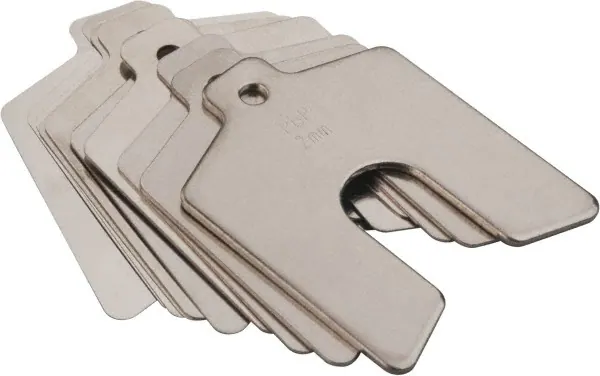
\includegraphics[scale=0.25]{Images/shims.png}
		\captionof{figure}{{\it Shims} of various thicknesses}
		\small\textsuperscript{Source: www.mscdirect.com/product/details/70475967}
		\label{fig:shims}
		
	\end{minipage}\hfill
	\begin{minipage}{0.58\linewidth}
		\scriptsize
		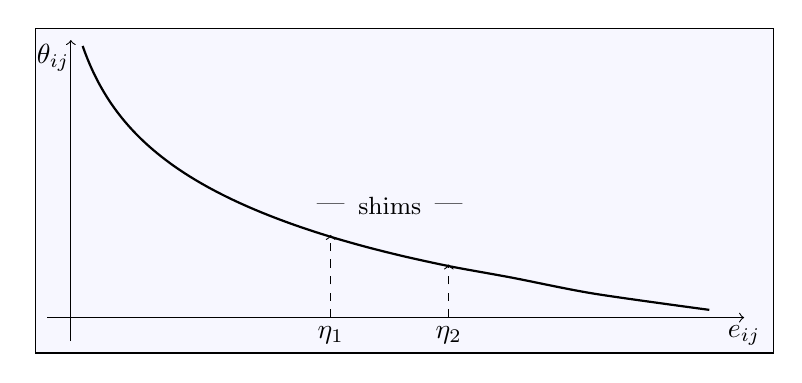
\begin{tikzpicture}[scale=0.75, samples=100]
			\filldraw[fill=blue!3!white, draw=black] (0, 0) rectangle (12.5, 5.5);
			\draw[->] (.2, .6) -- coordinate (x axis mid) (12, .6);
			\node at (5, 0.3) {$\eta_1$};
			\node at (5, 2.5) {|};
			\node at (6, 2.5) {\small{shims}};
			\node at (7, 2.5) {|};
			\node at (7, 0.3) {$\eta_2$};
			\node at (0.3, 5) {$\theta_{ij}$};
			\draw[->] (.6, .2) -- coordinate (y axis mid) (0.6, 5.3);
			\node at (12, 0.3) {$e_{ij}$};
			\draw[smooth, domain = 0.09:2, color=black, thick] plot (.3+1/\x,{4.2+log2(\x)});
			\draw[->, dashed] (5, 0.6)--(5, 2.0);
			\draw[->, dashed] (7, 0.6)--(7, 1.5);
		\end{tikzpicture}
		
		\captionof{figure}{$n_{\pi_k}$\/ possible edges $e_{ij}$\/ sorted by $\theta_{ij}$\/ in non-ascending order}
		\label{fig:whip}		
	\end{minipage}
\end{table}

Considering only the items that can be shipped at the node $\pi_k$, Figure \ref{fig:whip} represents $n_{\pi_k}$\/ possible edges $e_{ij}$\/ of the pallet $i$\/ sorted by $\theta_{ij}$\/ in non-ascending order. Initially, $Shims$\/ builds a greedy solution for the pallet $i$\/ selecting edges up to index $\eta_1$ (first phase). Then, with the edges between $\eta_1$\/ and $\eta_2$, it elaborates different possible complements (second phase), including later the best ones in the same pallet (third phase). $Shims$\/ is described in Algorithm \ref{alg:shims}. 




\begin{algorithm}[H]
	\caption{$Shims$\/ heuristic at the node $\pi_k$}  \label{alg:shims}
	\begin{algorithmic}[1]
		
		\Procedure{$SolveNode$}{$Shims, \pi_k, G, tmax$}
	
		\State $T_{begin} \gets$ current system time
	
		\State Let $G(M \cup N_{\pi_k} \cup Q_{\pi_k}, E_{Q_{\pi_k}})$   \label{shims:initQ}
		
		\State Sort $M$ by $|D_i^{long}|$ in non-descending order \label{shims:pallets}
		
		\State $E_{N_{\pi_k}} \gets \varnothing$  \Comment{An empty set of pallet-item edges}
				
		\State $\tau_{max} \gets W_{max} \times limit^{CG}_{long}$ \Comment{Maximum aircraft torque}

		\State $limit \gets 0.92$  \label{shims:limit}
		
		\For{$i \gets 1$ to $m$}  \label{shims:eta1_a}
							
			\State $\tau_{\pi_k} \gets \sum_{(i,q)\in E_{Q_{\pi_k}}} w_q \times D_i^{long}$ \Comment{Torque due to the packed contents}	
			\State $vol_i \gets \sum_{(i,q)\in E_{Q_{\pi_k}}} v_q$ \Comment{Volume at the pallet $i$\/ due to the packed contents}	
			
			\State Let $E$\/ be an array of $n_{\pi_k}$ possibles edges of the pallet $i$\/ sorted by $\theta_{ij}$\/ in non-ascending order \label{shims:possible}
			\State $\eta_1 \gets 1$  
			\Repeat
				\State $e_{ij} \gets E_{\eta_1}$ \Comment{$e_{ij}$\/ is the possible allocation of the item $j$\/ to the pallet $i$}
								
				\If{ ($E_{N_{\pi_k}} \cup \{e_{ij}\}$ is feasible) {\bf and} ($vol_i \leq V_i \times limit$) {\bf and} ($| \tau_{\pi_k} + w_j \times D_i^{long} | \leq W_{max} \times limit^{CG}_{long}$)} 
				
					\State $E_{N_{\pi_k}} \gets E_{N_{\pi_k}} \cup \{e_{ij}\}$
					
					\State $vol_i \gets vol_i + v_j$
					
					\State $\tau_{\pi_k} \gets \tau_{\pi_k} + w_j \times D_i^{long}$
					
					\State $\eta_1 \gets \eta_1 + 1$ 
				
				\EndIf
			\Until ($vol_i > V_i \times limit$) {\bf or} ($\eta_1>n_{\pi_k}$)		 \Comment{End of the first phase} \label{shims:endfirst}	
				

			\State $slack_i \gets V_i - vol_i$  \label{shims:beginsecond}
			\State $\eta_2 \gets \eta_1$  \label{shims:eta2a}
			\While{($\eta_2 \leq n_{\pi_k}$) {\bf and} ($ vol_i < (1 + 2 \times (1-limit)) \times V_i$)}

					\State $e_{ij} \gets E_{\eta_2}$
			
					\State $vol_i \gets vol_i + v_j$
					\State $\eta_2 \gets \eta_2 + 1$  \label{shims:eta2} \label{shims:endsecond} \Comment{End of the second phase}
			\EndWhile 
				
			
			\State $vol \gets 0$; $b \gets 1$; $shims_b \gets \varnothing$; $Set \gets \{ shims_b \}$  \label{shims:beginthird} 
			
		
			
			\For{$x \gets \eta_1$ to $\eta_2$} \label{edges_indexes}
				
				\If{ $T_{current} - T_{begin} > tmax$}
				\State {\bf break}  \Comment{Runtime limit exceeded}
				\EndIf
			
				\State $NewShims \gets$ {\bf True} \label{new_shims}
				\State $e_{ij} \gets E_x$
				
				\For{$shims \in Set$} \label{shims_set}
				
					\If {($e_{ij} \not\in (E_{N_{\pi_k}} \cup shims))$ {\bf and} ($e_{ij}$ is feasible)  {\bf and} ($(v_j + vol) \leq slack_i$)}
					
						\State $shims \gets shims \cup \{e_{ij}\}$
						\State $vol \gets vol + v_j$
						\State $NewShims \gets$ {\bf False} \label{new_shims_false}
						
						\State {\bf break}  
					\EndIf
				
				\EndFor 
			
				\If{$NewShims$} \label{new_shims2}
					\State $vol \gets 0$; $b \gets b + 1$;  $shims_b \gets \{e_{ij}\}$
					\State $Set \gets Set \cup \{ shims_b \}$
				\EndIf
			
			\EndFor 
			
			\State $sh_w \gets shims$, where $shims \in Set$ and $\sum_{e_{ij} \in shims} w_j$\/ is maximum  \label{best_weight}		
			\State $sh_v \gets shims$, where $shims \in Set$ and $\sum_{e_{ij} \in shims} v_j$\/ is maximum \label{best_volume}
			\State $sh_{best} \gets shims$, where $shims \in \{sh_w, sh_v\}$\/ and $\sum_{e_{ij} \in shims} s_j$\/ is maximum \label{best_score}
			\State $E_{N_{\pi_k}} \gets E_{N_{\pi_k}} \cup sh_{best}$ \label{shims:endthird}  \Comment{End of the third phase}

		\EndFor
		
		\Return $G(M \cup N_{\pi_k} \cup Q_{\pi_k}, E_{Q_{\pi_k}} \cup E_{N_{\pi_k}})$
		
		\EndProcedure
	\end{algorithmic}
\end{algorithm}

Initially, $Q_{\pi_k}$\/ (line \ref{shims:initQ}) corresponds to the packed contents that remain on board. It is important to remember that $E_{Q_{\pi_k}}$\/ and $M$\/ were modified by $UpdatePacked(M, Q_{\pi_k}, \pi_k)$ and $SetPalletsDestinations(M, \pi_k)$. Then, the pallets $i$\/ are considered in non-descending order of $|D_i^{long}|$. 

For each pallet $i$, its $n_{\pi_k}$\/ possible edges $e_{ij}$\/ are considered in non-increasing order of $\theta_{ij}$:

	
\begin{itemize}
	
	\item In {\it greedy phase}\/ (lines \ref{shims:pallets}-\ref{shims:endfirst}), a partial solution for each pallet $i$\/ is constructed by adding edges following $\theta_{ij}$\/ order. The $\eta_1$\/ index corresponds to the accumulated volume equal to $V_i \times limit$. In $\eta_2$\/ index, this same accumulated volume reaches $(1 + 2\times(1 - limit))\times V_i$. The size of this range $[\eta_1,\eta_2]$\/ was defined empirically, and the value $limit=0.92$\/ (line \ref{shims:limit}) was determined by the {\it iRace} tool \cite{LopezIbanezManuel2016}.
	
	\item In {\it composition phase}\/ (lines \ref{shims:beginsecond}-\ref{shims:endsecond}), a set of shims named $Set$\/ is created for each pallet $i$, where each shim is formed by a set of edges in the range $[\eta_1,\eta_2]$, whose total volume is limited by $slack_i$. In this phase, the heuristic that provided the best results, both in terms of time and quality, is based on {\it First-Fit Decreasing}, which is an approximation algorithm for the {\it Bin Packing Problem}\/ \cite{JohnsonGarey1985}. Basically, shims are created by accumulating the following edges, taking $slack_i$\/ as a limit.
	
	\item In {\it selection phase}\/ (lines \ref{shims:beginthird}-\ref{shims:endthird}), the best shim in $Set$\/ is chosen. Initially, two shims are found: $sh_w$\/ with larger weight, and $sh_v$\/ with larger volume. Between the two, the one with the highest score will be chosen and its edges are inserted into $E_{N_{\pi_k}}$.
	
\end{itemize}



\section{Implementation and results}
\label{sec6}

This section is composed of two parts: the generation of test instances and the results obtained in our implementation.


\subsection{Instances generation}
\label{items}

As we are dealing with a new problem, which until now had not been modeled in the literature, we have to create our own benchmarks. For this, we based on the characteristics of real airlifts carried out by the {\it Brazilian Air Force}, as described below.

In the military airlift carried out in Brazil from 2008 to 2010, 23\% of the items weighed between $10kg$ and $20kg$, 22\% from $21kg$ to $40kg$, 24\% from $41kg$ to $80kg$, 23\% from $81kg$ to $200kg$, and 8\% between $201kg$ and $340kg$. These five groups of items are described in Table \ref{tab:weights}, where $P$\/ represents the group probability. On the other hand, the average density of these items is approximately $246 kg/m^3$.

\begin{table}[H]
	\centering
	\caption{Items weight distribution}  \label{tab:weights}
	\begin{tabular}{c c c c }
		\toprule
		$Group$ & $P$ & $low$ ($kg$) & $high$ ($kg$) \\		
		\midrule
		1              & 0.23           & 10  & 20  \\
		2              & 0.22           & 21  & 40  \\
		3              & 0.24           & 41  & 80  \\		
		4              & 0.23           & 81  & 200 \\
		5              & 0.08           & 201 & 340 \\
		\bottomrule
	\end{tabular}
\end{table}


In the generation of test instances, we use three types of random selections:
\begin{itemize}
	\item $RandomReal(r_1,r_2)$: randomly selects a real number in $[r_1,r_2]$, where $r_1$ and $r_2$ are real numbers;
	\item $RandomInt(i_1,i_2)$: randomly selects a integer number in $[i_1,i_2]$, where $i_1$ and $i_2$ are integer numbers;
	\item $Roulette(set)$ biased through $\phi$: selects an element from $set$, where the probability of each element is proportional to the value of a given function $\phi$\/ defined on $set$.
\end{itemize}

$ItemsGeneration$, which generates $N$, is described in Algorithm \ref{alg:itemsgen}.

\begin{algorithm}[H]
	\caption{Generating items}  \label{alg:itemsgen}
	\begin{algorithmic}[1]
		
		\Procedure{$ItemsGeneration$}{$scenario, surplus$}
		\State Let $L$\/ and $M$  \Comment{From Tables \ref{tab:larger} and \ref{tab:scenarios}} \label{ig:LM}
		\State $limit \gets surplus \times \sum_{i=1}^{m} V_i$ \label{ig:extended}

		\For{$k \gets 0$ to $K$}
		
			\State $N_k \gets \varnothing$
			\State $j \gets 0$
			\State $vol \gets 0$	\label{ig:totals}	
			\While{$vol < limit$}
			
				\State $j \gets j+1$
				\State Let $t_j^k$\/ be the item $j$\/ at the node $k$
				\Repeat
					\State $to_j \gets RandomInt(0, K)$ \label{ig:dest}
				\Until{$to_j \neq k$}
				
				\State $x = Roulette(item)$ biased through $P$ \label{ig:weight1} \Comment{From Table \ref{tab:weights}}
					
				\State $w_j \gets RandomReal(low(x), high(x))$        \label{ig:weight2}		
				
				\State $s_j \gets \round{100 \times (1 - \log_{10}(RandomInt(1, 9)))} $ \label{ig:score}
				
				\State $v_j \gets w_j / RandomReal(148, 344)$ \label{ig:volume}
				
				\State $vol \gets vol + v_j$ 
				
				\State $N_k \gets N_k \cup \{t_j^k\}$ 
			\EndWhile

		\EndFor
		
		\State $N \gets \bigcup_{0 \leq k \leq K} N_k$
		
		\Return $N$
		
		\EndProcedure
	\end{algorithmic}
\end{algorithm}

$scenario$\/ defines $L$\/ and $M$\/ (line \ref{ig:LM}), and $surplus$\/ sets a limit on the total volume of items at each node (line \ref{ig:extended}). To avoid simply loading all items, we use $surplus \in \{1.2, 1.5, 2.0\}$. This also represents more instances for tests in each scenario.

For each generated $t^k_j$\/ item, its destination is randomly selected (line \ref{ig:dest}), its weight has a distribution according to Table \ref{tab:weights} (lines \ref{ig:weight1}-\ref{ig:weight2}), its score varies $100$\/ (highest) and $5$\/ (lowest) according to a logarithmic scale (line \ref{ig:score}, and its volume is randomly defined from the density, where we allow a variation of 40\% more or less than the average density of $246 kg/m^3$\/ (line \ref{ig:volume}).




\subsection{Results obtained}

In the tests performed, we used a 64-bit, 16GB, 3.6GHz, eight-core processor with {\it Linux Ubuntu 22.04.1 LTS 64-bit} as the operational system and {\it Python 3.10.4}\/ as the programming language. We also used the well-known solver $Gurobi$\/ ({\tt www.gurobi.com}), version 9.5.2.

We ran Algorithm \ref{alg:main} considering 5 values for $scenario$\/ from Table \ref{tab:scenarios}, 3 values for  $surplus$\/ from $\{1.2, 1.5, 2.0\}$, 4 values for $tmax$\/ from $\{240s, 1200s, 2400s, 3600s\}$, and 6 different $method$\/ for the node-by-node solution: $Gurobi$\/ (see \ref{solver}), ACO, NMO, TS, GRASP, and $Shims$\/ (Algorithm \ref{alg:shims}). 

In order for $Gurobi$\/ to be able to solve the largest possible number of tests without memory overflow, we set its parameter {\it MIPgap}\/ to 1\%. This shortens its runtime, in addition to ensuring that its objective function $f$\/ is at most 1\% of the optimal solution. For more details, see {\tt https://support.gurobi.com}.

Among the heuristics, we will present only the results obtained by $Shims$, which had the best performance. For each $scenario$, $surplus$\/ and $tmax$, 7 different instances were generated. We will present the average of the objective function $f$\/ and the runtime of $Gurobi$\/ and $Shims$\/ in these instances. To facilitate the comparison between both, we added a last column in the tables, where two values are indicated:
\begin{itemize}
	\item {\bf Normalized}: value between 0 and 1, which corresponds to the ratio between the sum of $f$\/ values obtained by the method in all scenarios and the sum of the best values obtained by both methods in all scenarios. The higher the value of {\bf Normalized}, the closer the method approached the best solutions found.
	\item {\bf Speed-up}: ratio of the sums of the runtimes of all scenarios and the sum of the method runtimes in all scenarios. The method with the highest {\bf Speed-up}\/ is the fastest.
\end{itemize}

We also indicate the two adopted strategies: dedicating all the processing time to the two shortest tours, or distributing it among all the $K!$\/ tours.

The results obtained with $tmax = 3600s$, which is the highest tested runtime limit, are in Tables \ref{tab:20}, \ref{tab:50} and \ref{tab:100}, with $surplus$\/ values $1.2$, $1.5$\/ and $2.0$, respectively. We indicate with an {\bf x} the cases where $Gurobi$\/ did not find a feasible solution within this runtime limit, or had to be aborted due to high RAM consumption.


\begin{table}[H]
	\centering
	\caption{Solutions with $surplus = 1.2$\/ and $tmax =  3600s$}  \label{tab:20}
	\footnotesize
	\begin{tabular}{ccccccccc}
		\toprule
		{\specialcell{{\bf Tested}\\{\bf tours}}}&$method$          & $scenario$ & {\bf 1} & {\bf 2} & {\bf 3} & {\bf 4} & {\bf 5} & \specialcell{{\bf Normalized}\\{\bf Speed-up}}   \\
		\toprule
		\multirow{4}{*}{Shortest} &\multirow{2}{*}{$Gurobi$} & $f$ & 8.52    & 11.70   & 13.07   & 13.54 & 12.44     &  1.00\\
		&                                                               &               {time (s)}  & 17      & 17      & 16      & 17    & 26        &  1.0 \\
		\cmidrule(lr){2-9}
		&                                                               \multirow{2}{*}{$Shims$}    & $f$ & 8.54    & 11.63   & 12.97   & 13.43 & 12.36     &  0.99 \\
		&                                                               &         {time (s)}        & 1       & 1       & 2       & 2     & 2         &  11.6 \\
		
		\midrule
		
		\multirow{4}{*}{All $K!$}&                                  \multirow{2}{*}{$Gurobi$} & $f$ & 8.52    & 12.25   & 13.32   & 14.61  & x        & 1.00 \\
		&                                                               &               {time (s)}  & 25      & 36      & 121     & 297    & x        &  1.0 \\
		\cmidrule(lr){2-9}	
		&                                                               \multirow{2}{*}{$Shims$}    & $f$ & 8.54    & 12.26   & 13.23   & 14.53  & 13.42    & 0.99  \\
		&                                                               &         {time (s)}        & 1       & 2       & 6       & 17     & 106      & 18.4   \\
		\bottomrule
		
	\end{tabular}
	\normalsize
\end{table}


\begin{table}[H]
	\centering
	\caption{Solutions with $surplus = 1.5$\/ and $tmax =  3600s$}  \label{tab:50}
	\footnotesize
	\begin{tabular}{ccccccccc}
		\toprule
		{\specialcell{{\bf Tested}\\{\bf tours}}} & $method$          & $scenario$ & {\bf 1} & {\bf 2} & {\bf 3} & {\bf 4} & {\bf 5} & \specialcell{{\bf Normalized}\\{\bf Speed-up}}   \\
		\toprule
		\multirow{4}{*}{ Shortest } & \multirow{2}{*}{$Gurobi$} & $f$ & 11.80 & 16.74 & 18.04 & 18.86 & 16.92 & 1.00 \\
		&&               {time (s)}                                                                  & 38    & 30    & 27    & 29    & 81    & 1.00  \\
		\cmidrule(lr){2-9}	
		&\multirow{2}{*}{$Shims$}                                                                    & $f$ & 11.83 & 16.74 & 18.01 & 18.89 & 16.91 & 1.00  \\
		&&         {time (s)}                                                                        & 1     & 2     & 2     & 3     & 3     & 20.5  \\
		
		\midrule
		
		\multirow{4}{*}{All $K!$} & \multirow{2}{*}{$Gurobi$}                                  & $f$ & 11.81 & 17.01 & 18.25 & 20.59 & 18.36   & 1.00 \\ 
		&&               {time (s)}                                                                  & 53    & 61    & 193   & 470   & 2241    & 1.0  \\
		\cmidrule(lr){2-9}	
		&\multirow{2}{*}{$Shims$}                                                                    & $f$ & 11.83 & 17.00 & 18.21 & 20.45 & 18.00   & 0.99  \\ 
		&&         {time (s)}                                                                        & 1     & 2     & 9     & 26    & 157     & 15.5 \\
		\bottomrule
		
	\end{tabular}
	\normalsize
\end{table}


\begin{table}[H]
	\centering
	\caption{Solutions with $surplus = 2.0$\/ and $tmax =  3600s$}  \label{tab:100}
	\footnotesize
	\begin{tabular}{ccccccccc}
		\toprule
		{\specialcell{{\bf Tested}\\{\bf tours}}}& $method$          & $scenario$ & {\bf 1} & {\bf 2} & {\bf 3} & {\bf 4} & {\bf 5} & \specialcell{{\bf Normalized}\\{\bf Speed-up}}   \\
		\toprule
		\multirow{4}{*}{Shortest} & \multirow{2}{*}{$Gurobi$} & $f$ & 17.75 & 24.39 & 26.46 & 27.09 & 24.00 & 1.00 \\ 
		&&                                                                               {time (s)}  & 162   & 95    & 74    & 68    & 67    & 1.0  \\
		\cmidrule(lr){2-9}	
		&                                                                   \multirow{2}{*}{$Shims$} & $f$ & 17.78 & 24.40 & 26.36 & 27.01 & 23.94 & 0.99  \\
		&&                                                                                {time (s)} & 2     & 3     & 3     & 4     & 5     & 27.4  \\
		
		\midrule
		
		\multirow{4}{*}{All $K!$} & \multirow{2}{*}{$Gurobi$} & $f$ & 17.75 & 25.24 & 26.46 & 29.11 &  x   & 1.00 \\ 
		&&                                                                                {time (s)} & 151   & 123   & 319   & 689   &  x   & 1.0  \\
		\cmidrule(lr){2-9}	
		&                                                                \multirow{2}{*}{$Shims$}    & $f$ & 17.78 & 25.25 & 26.38 & 28.98 & 26.08 & 1.00  \\
		&&                                                                                {time (s)} & 2     & 3     & 13    & 37    & 229   & 23.3  \\
		\bottomrule
		
	\end{tabular}
	\normalsize
\end{table}


From these data, we can make some conclusions:
\begin{itemize}
\item The strategy of testing all $K!$\/ tours often gives a better quality solution.
\item $Gurobi$\/ fails in some cases, when $scenario=5$\/ and the strategy is to check all $K!$\/ tours. This occurs because the runtime limit per node is smaller, and there tends to be more packed contents on the aircraft, reducing the space for allocating items and making the solution difficult.
\item When $Gurobi$\/ finishes, it finds the best solution, but the one obtained by $Shims$\/ reaches $99\%$\/ of that value.
\item $Shims$\/ always finds a solution, being 11 to 27 times faster.
\item All runtimes are much lower than the limit because the solution on many nodes can be fast. Anyway, in all the tests performed, the maximum time spent by $Shims$\/ did not reach 4 minutes, that is, it is practically instantaneous. On the other hand, when $scenario=5$\/ and $surplus=1.5$, Gurobi spent almost 40 minutes.
\end{itemize}

Table \ref{tab:100time} shows the results obtained with the strategy of testing the $K!$\/ tours in all scenarios with different runtime limits. We can observe more cases where $Gurobi$\/ fails, even in smaller scenarios. When $Gurobi$\/ finishes, $Shims$\/ finds quickly a solution of similar quality ($98\%$\/ or better). In all cases, $Shims$\/ finds a good solution in less than 4 minutes.


\begin{table}[H]
	\centering
	\caption{Solutions testing all $K!$\/ tours with different runtime limits}  \label{tab:100time}
	\scriptsize
	\setlength{\tabcolsep}{3.5pt}
	\begin{tabular}{ccc|ccccc|ccccc|ccccc}
		\toprule
		&             \multicolumn{2}{r}{$surplus$} &\multicolumn{5}{c}{\bf 1.2}&\multicolumn{5}{c}{\bf 1.5}&\multicolumn{5}{c}{\bf 2.0} \\
		\midrule
		$method$& {$tmax$} & $scenario$  &{\bf 1}&{\bf 2}&{\bf 3}&{\bf 4}&{\bf 5}&{\bf 1}&{\bf 2}&{\bf 3}&{\bf 4}&{\bf 5}&{\bf 1}&{\bf 2}&{\bf 3}&{\bf 4}&{\bf 5} \\
		\toprule
		
		\multirow{10}{*}{$Gurobi$} & \multirow{2}{*}{240s} & $f$ & 8.53 & 12.24 & 13.34 &  x      &  x      & 11.81 & 17.02 & 18.31 &  x      &  x      & 17.75 & 25.24 & x     & x       & x \\ 
		&               &  {time (s)}                              & 41   & 43    & 123   &  x      &  x      & 50    & 62    & 181   &  x      &  x      & 166   & 140   & x     & x       & x \\ 
		\cmidrule(lr){2-18}		
		
		&                              \multirow{2}{*}{1200s} & $f$ & 8.52 & 12.25 & 13.31 & 14.67   & x       & 11.81 & 17.02 & 18.25 &  20.64  &  x      & 17.75 & 25.24 & 26.49 & 27.97   & x \\ 
		&        &  {time (s)}                             & 39   & 41    & 129   & 217     & x       & 52    & 61    & 190   &  304    &  x      & 161   & 139   & 384   & 579     & x \\ 
		\cmidrule(lr){2-18}                              
		& \multirow{2}{*}{2400s}& $f$                               & 8.53 & 12.25 & 13.30 & 14.59   & 13.59   & 11.80 & 17.02 & 18.25 &  20.60  &  x      & 17.75 & 25.24 & 26.46 & 29.10   & x \\
		&        &  {time (s)}                             & 33   & 39    & 127   & 313     & 1444    & 51    & 62    & 188   &  327    &  x      & 158   & 127   & 381   & 543     & x \\
		\cmidrule(lr){2-18}                              		
		
		& \multirow{2}{*}{3600s}& $f$                               & 8.52 & 12.25 & 13.32 & 14.61   & x       & 11.81 & 17.01 & 18.25 &  20.59  & 18.36   & 17.75 & 25.24 & 26.46 & 29.11   & x \\ 
		&        &  {time (s)}                             & 25   & 36    & 121   & 297     & x       & 53    & 61    & 193   &  470    & 2241    & 151   & 123   & 319   & 689     & x \\ 
		
		\midrule
		
		\multirow{2}{*}{$Shims$} & \multirow{2}{*}{240s}  & $f$ & 8.54 & 12.26 & 13.23 & 14.53   & 13.42   & 11.83 & 17.00 & 18.21 &  20.45  & 18.00   & 17.78 & 25.25 & 26.38 & 28.98   & 26.08 \\ % 
		&         & {time (s)}                             & 1    & 2     & 6     & 17      & 109     & 1     & 2     & 8     &  26     & 160     & 2     & 3     & 13    & 37      & 229   \\ 
		
		\bottomrule
	\end{tabular}
	\normalsize
\end{table}


Most of $Gurobi$\/ executions consumed over 12 GB of RAM memory. Considering that the computer used in the experiments has a standard RAM consumption when idle of 3.5 GB (with {\it Python Interface Development Environment}, a PDF viewer, a system monitor, and a \LaTeX\/ IDE simultaneously open), the actual RAM consumption of $Gurobi$\/ was over 8.5 GB. On the other hand, all $Shims$\/ executions consumed at most 1.5 GB of RAM memory.


\section{Conclusions}
\label{sec7}

In this work, we modeled and solved a real air transport problem, named {\it Air Cargo Load Planning with Routing, Pickup and Delivery Problem}\/ (ACLP+RPDP). For the first time in the literature, a {\it NP-hard}\/ problem that involves {\it simultaneously}\/ pallet assembly, load balancing and route planning is addressed, where the cost-effectiveness of transport is maximized. We adopted some simplifications that are not critical, but that allowed the unprecedented solution of this problem considering more than two nodes.

We consider that, in practical cases, the number $K$\/ of nodes, excluding the base, is small ($K \leq 6$), each of them with hundreds of items to be shipped. Thus, considering a real aircraft, we have developed some node-by-node solutions, which are not necessarily optimal. This allows us to test two strategies: find a solution using the shortest tours, or enumerate all $K!$\/ tours and choose the best. The complete process can be executed quickly on a simple handheld computer, offering good results and reducing stress for the transport planners. As validation, we performed tests in several scenarios with real data from the {\it Brazilian Air Force}. At the moment, there is no commercial software available for this problem.

We have developed a solution process that, in less than 4 minutes, can establish a flight plan for a single aircraft with a good distribution of load on pallets to be put in the cargo bay, enforcing the loaded aircraft balance, maximizing the total score and minimizing fuel consumption. The output, which includes the tour plan and the pallet building and arrangement plan, is an essential part of airlift: it improves flight safety, makes ground operations more efficient, and makes sure that each item gets to its right destination. In this way, at each node of the tour, the time required is restricted exclusively to handling the airport equipment.

Our main contributions were the mathematical modeling of ACLP+RPDP that involves four sub-problems {\it NP-hard}\/, a complete process to solve it on a simple handheld computer, and a new heuristic that offers fast node solutions with good quality. Finally, by focusing on the node-to-node solution, the method of this work is not exclusive to aircraft and airports: it can be adapted, for example, to ships and ports, or vehicles and warehouses, or wagons and railways, provided that their practical cases are similar to those considered here. In these situations, it would be necessary to make some changes in the modeling: for example, modify the load balancing constraints, and consider the available space in vehicles or wagons instead of pallets.

As this is an ongoing research, we thought about some possible future improvements:
\begin{itemize}
\item consider a aircraft fleet, rather than a single one;
\item model three-dimensional items;
\item discard the highest cost tours, to reduce the runtime;
\item implement parallel algorithms in some steps of the solution.
\end{itemize}

\section*{References}

\begin{thebibliography}{00}

\bibitem{Karp1972} R. Karp, {\it Reducibility among combinatorial problems. Complexity of Computer Computations.} (R.E. Miller and J.M. Thatcher, eds.), Plenum Press, 85-103 (1972).

\bibitem{LarsenMikkelsen1979} O. Larsen and G. Mikkelsen, An interactive system for the loading of cargo aircraft, {\it European Journal of Operational Research}, Vol. 4 (6), pp. 367-373, 1980.

\bibitem{Brosh1981} Israel Brosh, Optimal cargo allocation on board a plane: a sequential linear programming approach, {\it European Journal of Operational Research}, Vol. 8 (1), pp. 40-46, 1981.

\bibitem{JohnsonGarey1985} D.S. Johnson and M.R. Garey, A 71/60 theorem for bin packing, {\it Journal of Complexity}, Vol. 1 (1), pp. 65-106, 1985.

\bibitem{Glover1986} Fred Glover, Future paths for integer programming and links to artificial intelligence, {\it Computers and Operations Research}, Vol. 13, pp. 533-549, 1986.

\bibitem{FeoResende1989} Thomas A. Feo and Mauricio G.C. Resende, A probabilistic heuristic for a computationally difficult set covering problem, {\it Operations Research Letters}, Vol. 8 (2), pp. 67-71, 1989.

\bibitem{Kevin1992} Kevin Y.K. Ng, A multicriteria optimization approach to aircraft loading, {\it Operations Research}, Vol. 40 (6), pp. 1200-1205, 1992.

\bibitem{Dorigo1992} Marco Dorigo, {\it Optimization, Learning and Natural Algorithms}, PhD Thesis, Politecnico di Milano, 1992.

\bibitem{CharonHudry1993} I. Charon and O. Hudry, The noising method: a new method for combinatorial optimization, {\it Operations Research Letters}, Vol. 14 (3), pp. 133-137, 1993.

\bibitem{DorigoManiezzoColorni1996} M. Dorigo, V. Maniezzo and A. Colorni, The ant system: optimization by a colony of cooperating agents, {\it IEEE Transactions on Systems, Man, and Cybernetics}, Vol. 26 (1), pp. 29-41, 1996.

\bibitem{NiarFreville1997} S. Niar and A. Freville, A parallel tabu search algorithm for the 0-1 multidimensional knapsack problem, Proceedings of {\it 11th International Parallel Processing Symposium}, 1997.

\bibitem{Heidelberg1998} K.R. Heidelberg, G.S. Parnell and J.E. Ames, Automated air load planning, {\it Naval Research Logistics}, Vol. 45 (8), pp. 751-768, 1998.

\bibitem{CharonHudry2001} I. Charon and O. Hudry, The noising methods: a generalization of some metaheuristics, {\it European Journal of Operational Research}, Vol. 135 (1), pp. 86-101, 2001.

\bibitem{MongeauBes2003} M. Mongeau and C. Bes, Optimization of aircraft container loading, {\it IEEE Transaction on Aerospace and Electronic Systems}, Vol. 39 (1), pp. 140-150, 2003.

\bibitem{fok2004optimizing} M.K.K. Fok and A.H.W. Chun, Optimizing air cargo load planning and analysis, Proceedings of {\it The International Conference on Computing, Communications and Control Technologies}, 2004.

\bibitem{Fidanova2006} S. Fidanova, Ant colony optimization and multiple knapsack problem and model bias, {\it Numerical Analysis and Its Applications}, Springer Berlin Heidelberg, pp. 280-287, 2005.

\bibitem{Chan2006} F.T.S. Chan, R. Bhagwat, N. Kumar. M.K. Tiwari and P. Lam, Development of a decision support system for air-cargo pallets loading problem: a case study, {\it Expert Systems with Applications}, Vol. 31 (3), pp. 472-485, 2006.

\bibitem{KaluznyBohdanL2009Oalb} B.L. Kaluzny and R.H.A.D. Shaw, Optimal aircraft load balancing, {\it International Transactions in Operational Research}, Vol. 16 (6), pp. 767-787, 2009.

\bibitem{MesquitaCunha2011} A.C.P. Mesquita and C.B. Cunha, An integrated heuristic based on the Scatter Search metaheuristic for vehicle routing problems with simultaneous delivery and pickup in the context of the Brazilian Air Force, {\it Transportes}, Vol. 19, pp. 33-42, 2011.

\bibitem{Verstichel2011} J. Verstichel, W. Vancroonenburg, W. Souffriau and G.V. Berghe, A mixed integer programming approach to the aircraft weight and balance problem, {\it Procedia Social and Behavioral Sciences}, Vol. 20, pp. 1051-1059, 2011.

\bibitem{Limbourg2012} S. Limbourg, M. Schyns and G. Laporte, Automatic aircraft cargo load planning, {\it Journal of the Operational Research Society}, Vol. 63 (9), pp. 1271-1283, 2012.

\bibitem{RoesenerHall2014} A.G. Roesener and S. Hall, A nonlinear integer programming formulation for the airlift loading problem with insufficient aircraft, {\it Journal of Nonlinear Analysis and Optimization: Theory and Applications}, Vol. 5 (1), pp. 125-141, 2014.

\bibitem{Vancroonenburg2014} W. Vancroonenburg, J. Verstichel, K. Tavernier and G.V. Berghe, Automatic air cargo selection and weight balancing: a mixed integer programming approach, {\it Transportation Research Part E: Logistics and Transportation Review}, Vol. 65, pp. 70-83, 2014.

\bibitem{LurkinSchyns2015} V. Lurkin and M. Schyns, The airline container loading problem with pickup and delivery, {\it European Journal of Operational Research}, Vol. 244 (3), pp. 955-965, 2015.

\bibitem{Feng2015} Feng, B.; Li, Y.; Shen, Z.J.M. {\it Air cargo operations: Literature review and comparison with practices.} Transp. Res. Part C Emerg. Technol. 2015, 56, 263?280. 

\bibitem{RoesenerBarnes2016} A.G. Roesener and J.W. Barnes, An advanced tabu search approach to the dynamic airlift loading problem, {\it Logistics Research}, Vol. 9 (1), pp. 1-18, 2016.

\bibitem{PaquaySchynsLimbourg2016} C. Paquay, M. Schyns and S. Limbourg, A mixed integer programming formulation for the three-dimensional bin packing problem deriving from an air cargo application, {\it International Transactions in Operational Research}, Vol. 23 (1-2), pp. 187-213, 2016.

\bibitem{PaquayLimbourgSchynsOliveira2018} C. Paquay, S. Limbourg, M. Schyns and J.F. Oliveira, MIP-based constructive heuristics for the three-dimensional bin packing problem with transportation constraints, {\it International Journal of Production Research},
Vol. 56 (4), pp. 1581-1592, 2018.

\bibitem{Laabadi2018} S. Laabadi, M. Naimi, H. El Amri and B. Achchab, The 0/1 multidimensional knapsack problem and its variants: a survey of practical models and heuristic approaches, {\it American Journal of Operations Research}, Vol. 8, pp. 395-439, 2018.

\bibitem{YangLiuGao2018} Y. Chenguang, L. Hu and G. Yuan, Load planning of transport aircraft based on hybrid genetic algorithm, {\it MATEC Web of Conferences}, Vol. 179, pp. 1-6, 2018.

\bibitem{Alonso2019} M.T. Alonso, R. Alvarez-Valdes and F. Parreno, A GRASP algorithm for multi-container loading problems with practical constraints, {\it A Quarterly Journal of Operations Research}, Vol. 18, pp. 49-72, 2019.

\bibitem{BrandtStefan2019} F. Brandt and S. Nickel, The air cargo load planning problem - a consolidated problem definition and literature review on related problems, {\it European Journal of Operational Research}, Vol. 275 (2), pp. 399-410, 2019.

\bibitem{wong2020} E.Y.C. Wong and K.K.T. Ling, A mixed integer programming approach to air cargo load planning with multiple aircraft configurations and dangerous goods, Proceedings of {\it 7th International Conference on Frontiers of Industrial Engineering}, 2020.

\bibitem{Zhan2020} S. Zhan, L. Wang, Z. Zhang and Y. Zhong, Noising methods with hybrid greedy repair operator for 0-1 knapsack problem, {\it Memetic Computing}, Vol. 12, pp. 37-50, 2020.

\bibitem{eugene2021} E.Y.C. Wong, D.Y. Mo and S. So, Closed-loop digital twin system for air cargo load planning operations, {\it International Journal of Computer Integrated Manufacturing}, Vol. 34 (7-8), pp. 801-813, 2021.

\bibitem{zhao2021} X. Zhao, Y. Yuan, Y. Dong and R. Zhao, Optimization approach to the aircraft weight and balance problem with the centre of gravity envelope constraints, {\it IET Intelligent Transport Systems}, Vol. 15 (10), pp. 1269-1286, 2021.

\bibitem{zhao2023} Zhao, Xiangling, Yun Dong, and Lei Zuo. {\it A Combinatorial Optimization Approach for Air Cargo Palletization and Aircraft Loading.} Mathematics (Basel) 11.13 (2023): 2798. Web.

\bibitem{LopezIbanezManuel2016} M. L�pez-Ib��ez, J. Dubois-Lacoste, L.P. C�ceres, M. Birattari and T. St�tzle, The irace package: Iterated racing for automatic algorithm configuration, {\it Operations Research Perspectives}, Vol. 3, pp. 43-58, 2016.


\end{thebibliography}


\end{document}




